\documentclass[xcolor=dvipsnames]{beamer}
\usepackage[T1]{fontenc}
\usepackage[utf8]{inputenc}
\usepackage[english,slovak]{babel}

\usepackage{amsmath}
\usepackage{amsthm}
\usetheme{Pittsburgh}
\useoutertheme{shadow}

\usepackage{graphicx}
\usepackage{caption}
\usepackage{subcaption}

\usepackage[]{algorithm2e}
\usepackage{listings}
 \setbeamercovered{transparent}
 \usepackage{cuted}
\usepackage[export]{adjustbox}
\usepackage{mathtools}

\usepackage{lipsum}
\usepackage{verbatim}
\usepackage{transparent}
\usepackage{framed}
\usepackage{xcolor}

\usepackage{multirow}
\usepackage{colortbl}
\usepackage{lmodern}

\usepackage{movie15}
\usepackage{media9}
\usepackage{verbatim}

\usepackage{animate}


\usepackage{hyperref}

\newcommand\Wider[2][3em]{%
\makebox[\linewidth][c]{%
  \begin{minipage}{\dimexpr\textwidth+#1\relax}
  \raggedright#2
  \end{minipage}%
  }%
}






\iftrue

\usetheme{Warsaw}

\setbeamercolor{normal text}{fg=white,bg=black!90}
\setbeamercolor{structure}{fg=white}

\setbeamercolor{alerted text}{fg=red!85!black}

\setbeamercolor{item projected}{use=item,fg=black,bg=item.fg!35}

\setbeamercolor*{palette primary}{use=structure,fg=structure.fg}
\setbeamercolor*{palette secondary}{use=structure,fg=structure.fg!95!black}
\setbeamercolor*{palette tertiary}{use=structure,fg=structure.fg!90!black}
\setbeamercolor*{palette quaternary}{use=structure,fg=structure.fg!95!black,bg=black!80}

\setbeamercolor*{framesubtitle}{fg=white}

\setbeamercolor*{block title}{parent=structure,bg=black!60}
\setbeamercolor*{block body}{fg=black,bg=black!10}
\setbeamercolor*{block title alerted}{parent=alerted text,bg=black!15}
\setbeamercolor*{block title example}{parent=example text,bg=black!15}

\fi



%-------------------------------------------------------------------------------------
\title{\color{white} \bf reinforcement learning introduction}
\author{\color{white} Michal CHOVANEC, PhD}


%\setbeamertemplate{footline}[frame number]{}
\setbeamertemplate{navigation symbols}{}


\date[EURP]{}
\begin{document}

{
    \usebackgroundtemplate
    {
        \vbox to \paperheight{\vfil\hbox to \paperwidth{\hfil

        {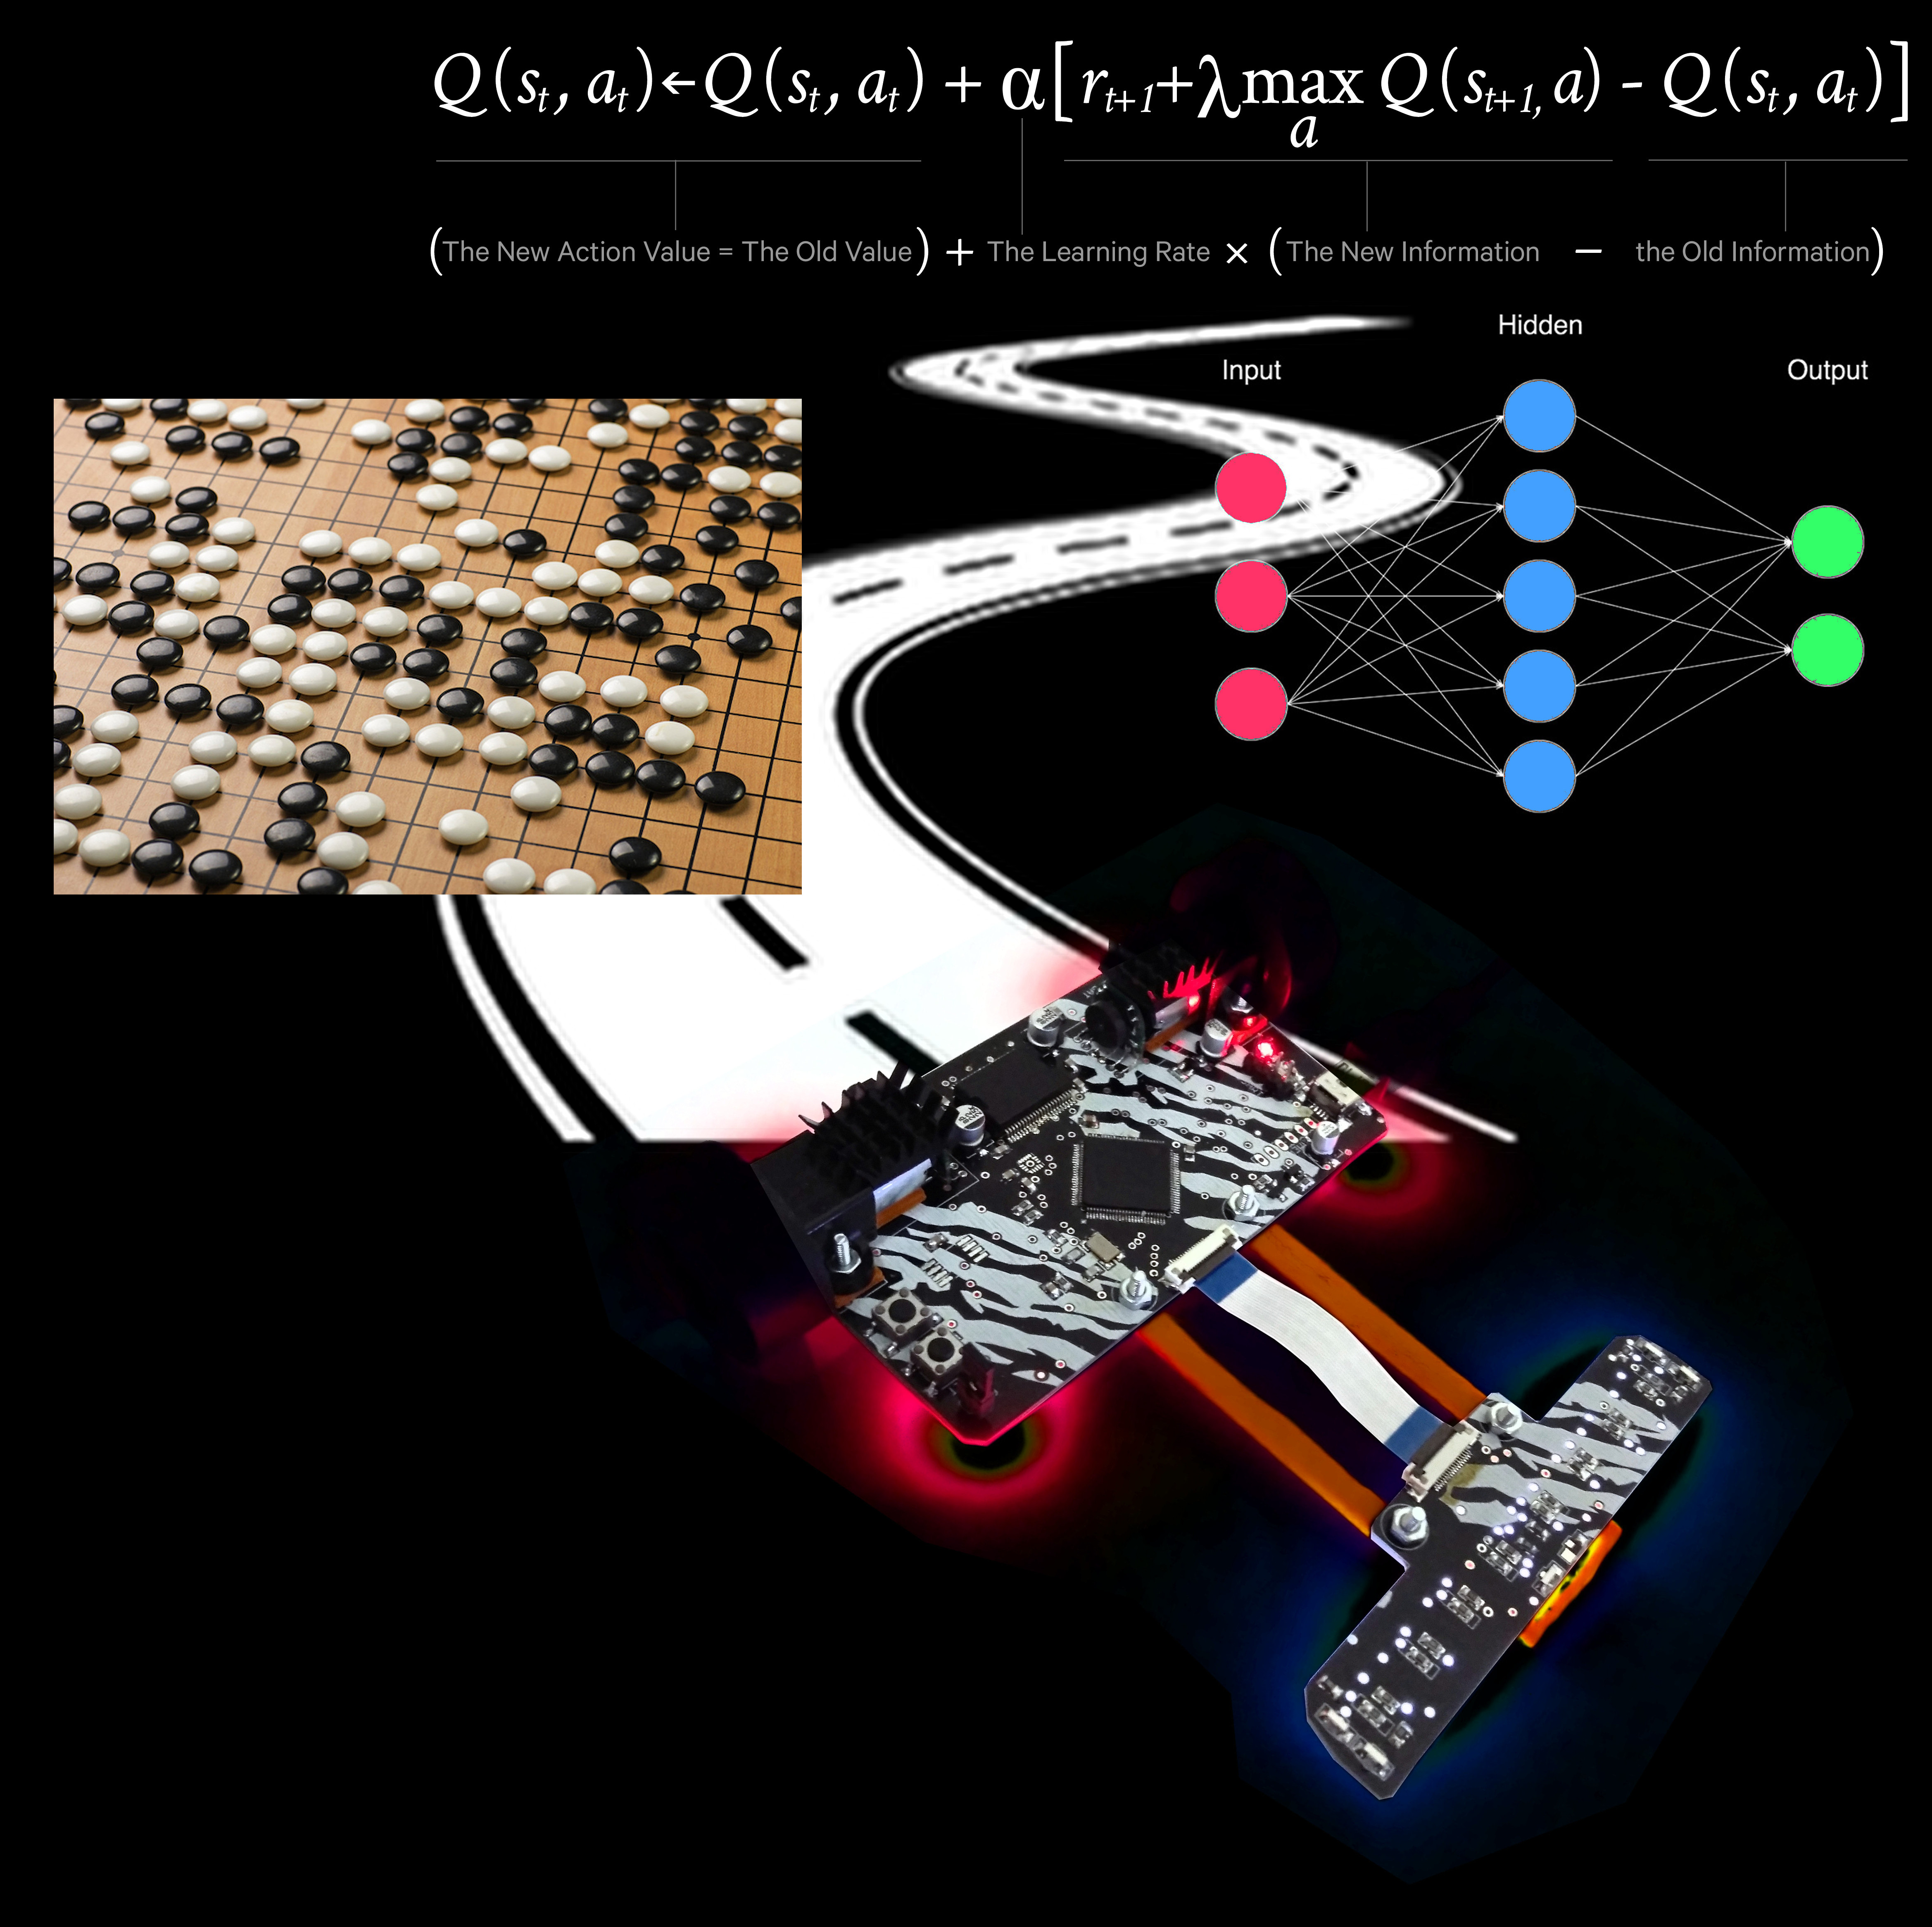
\includegraphics[width=5.05in]{../images/rl_square.jpg}}

        \hfil}\vfil}
    }



    \begin{frame}

    \centering
     \colorbox{black}
     {
        \begin{minipage}{8cm}
           {\LARGE \color{white}reinforcement learning -\\introduction} \\
           {\LARGE \color{white}Michal CHOVANEC, PhD.} \\
       \end{minipage}
     }

    \end{frame}
}



\begin{frame}{\bf Overview}

  \begin{enumerate}
      \item Agents - Principle
      \item Example problem - Drone Racing
      \item Policy Gradients -  Advantage-Actor-Critic (A2C)
      \item Practical Example - Lunar Lander
      \item Cookbook and Literature
  \end{enumerate}

  \centering{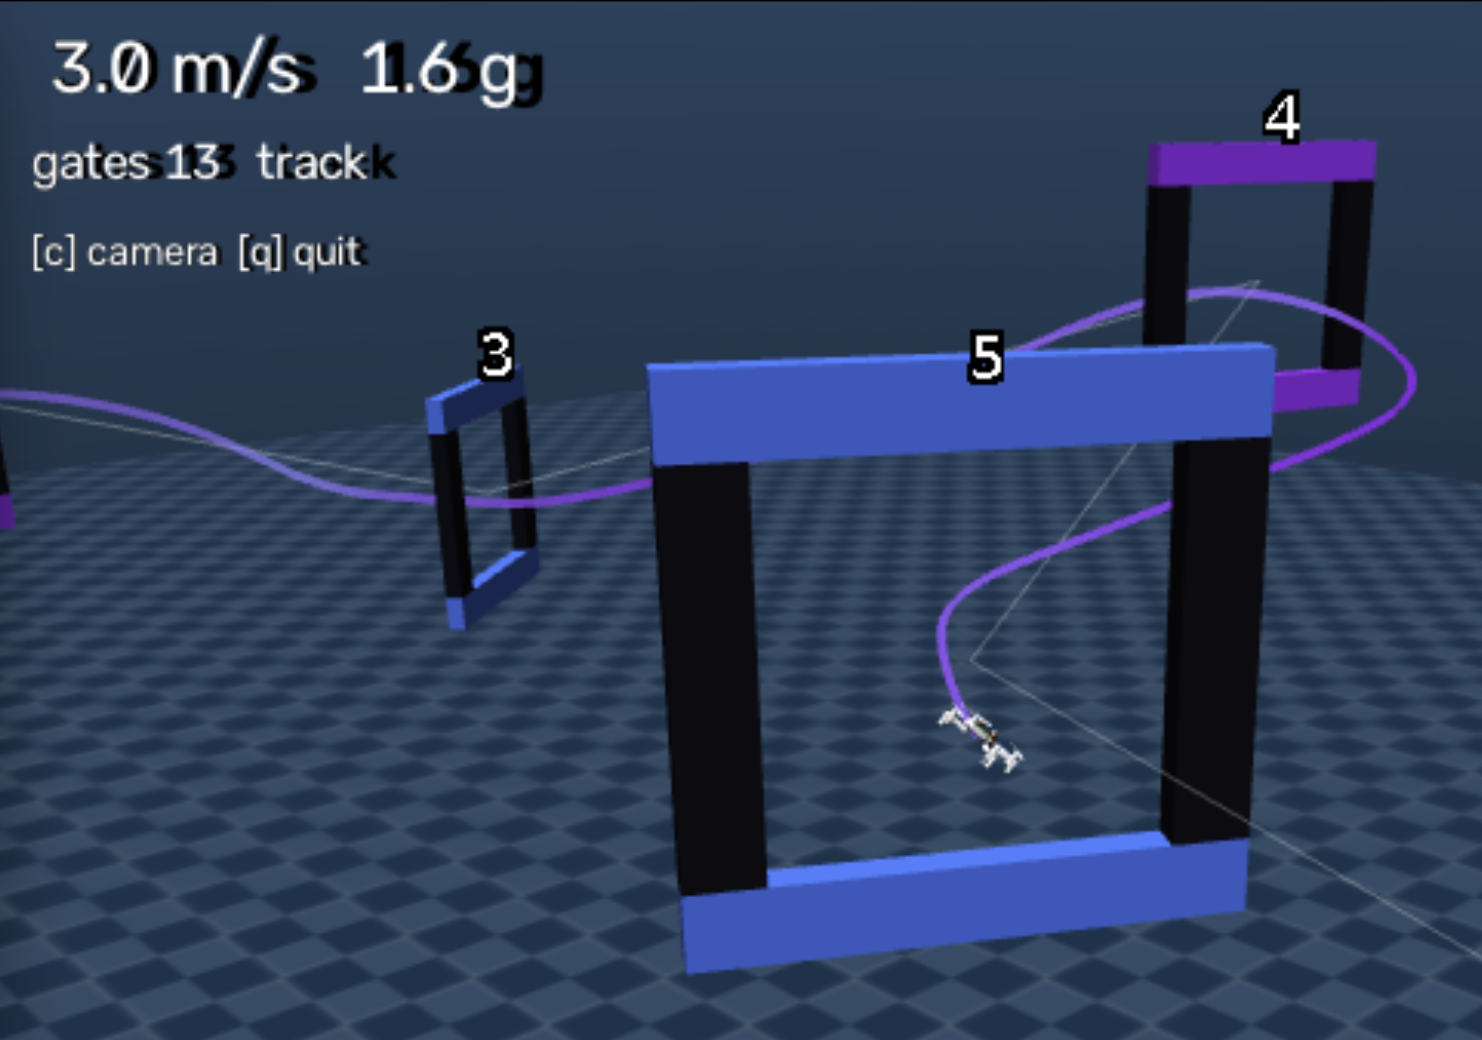
\includegraphics[scale=0.25]{../images/drone_race_2.png}}

\end{frame}



\begin{frame}{\bf Reinforcement learning}

  \begin{columns}

    \begin{column}{0.5\textwidth} 
      \centering{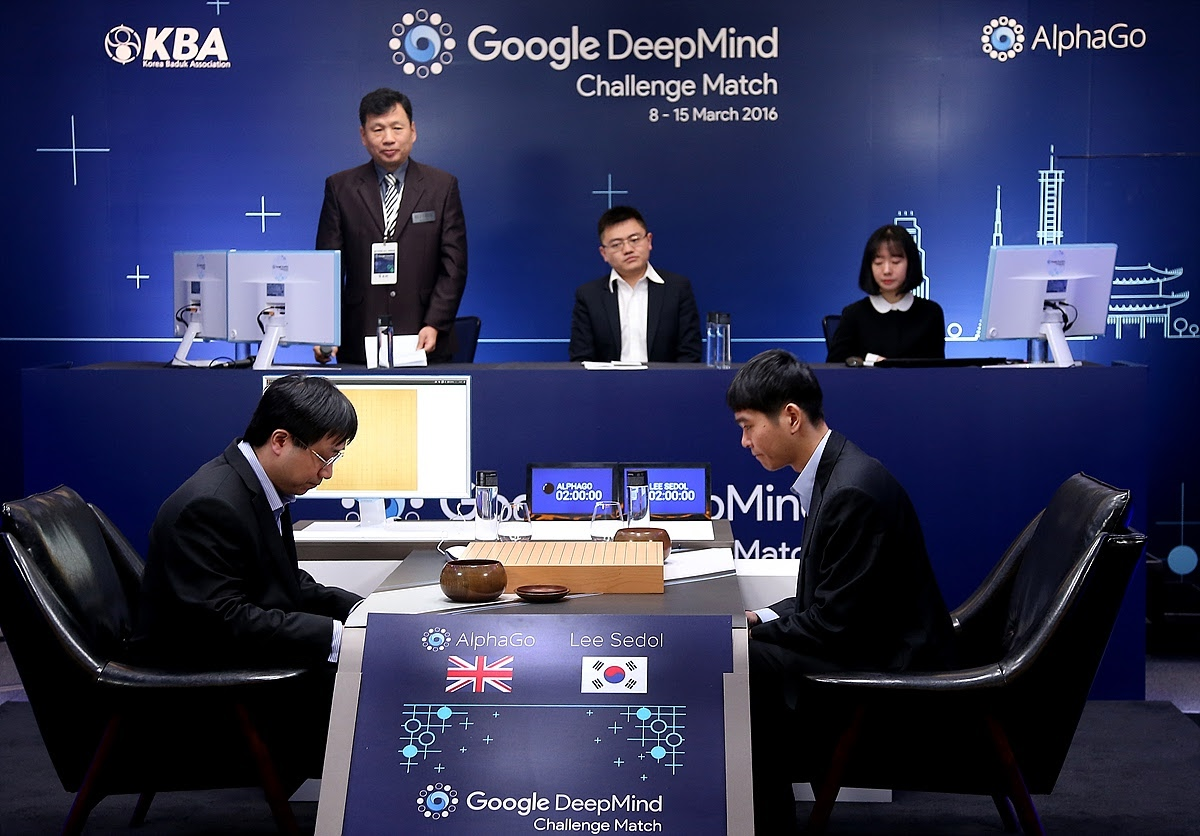
\includegraphics[scale=0.15]{../images/alpha_go.jpg}}
    \end{column} 
    \begin{column}{0.5\textwidth}
      \centering{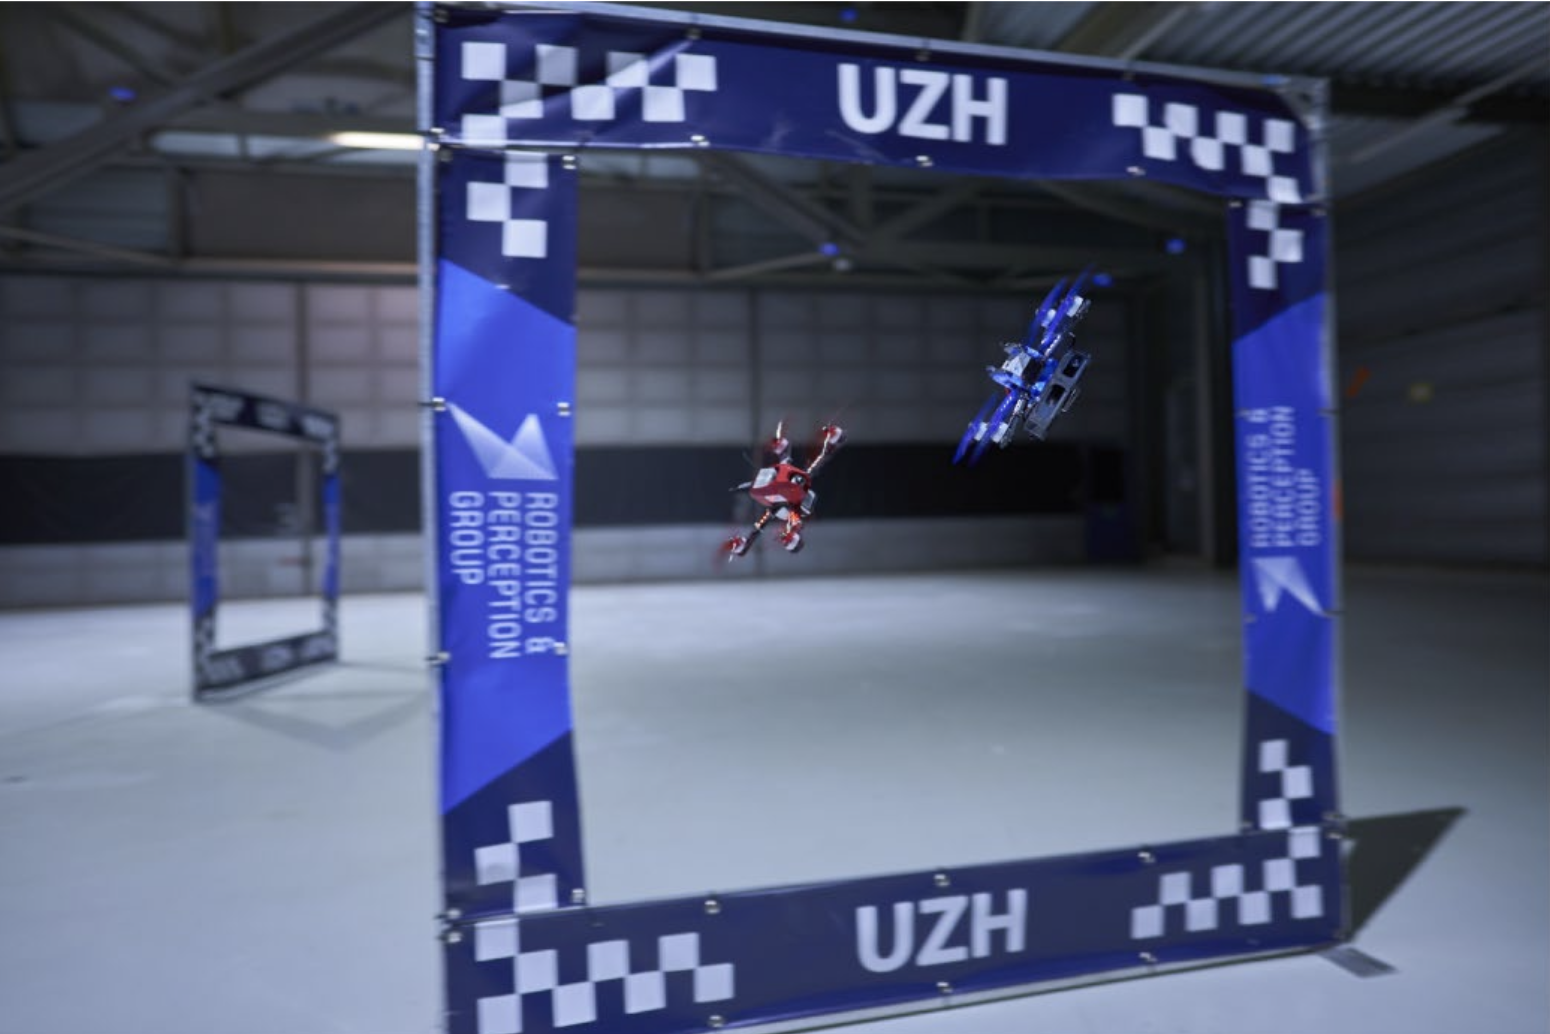
\includegraphics[scale=0.25]{../images/eth_drone.png}}
    \end{column}

  \end{columns}

\end{frame}



\begin{frame}{\bf Reinforcement learning - begining, 2013}

  \begin{columns}

    \begin{column}{0.5\textwidth} 
      \centering{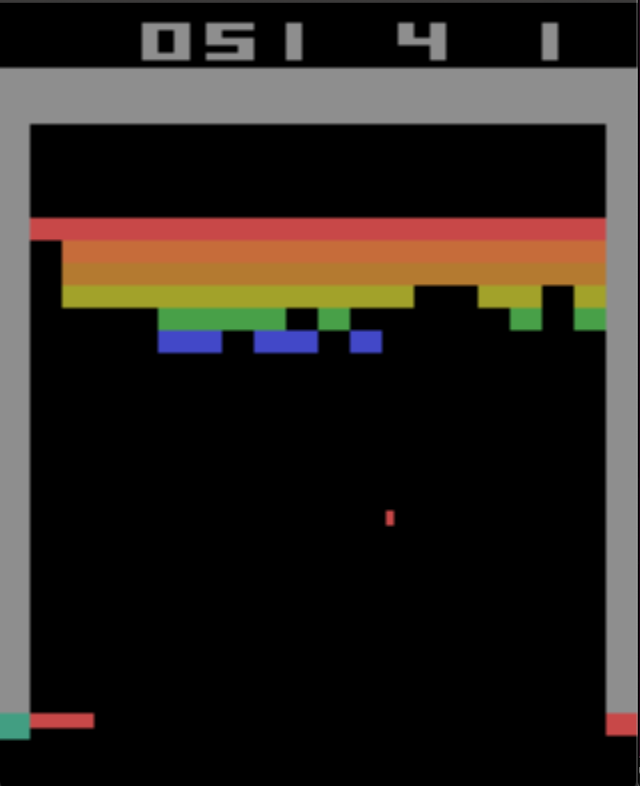
\includegraphics[scale=0.4]{../images/breakout.png}}
    \end{column} 
    \begin{column}{0.5\textwidth}
      \begin{itemize}
        \item \textbf{Playing Atari with Deep Reinforcement Learning}
        \item human level gameplay from screen osbservation
        \item Deep Q networks (DQN)
        \item tiny model : \\ 8x8x16 - 4x4x16 - 256 - output
      \end{itemize}
      
    \end{column}

  \end{columns}

\end{frame}



\begin{frame}{AlphaGo: Reinforcement Learning Beyond Human Play}
    \begin{columns}[T]
        \column{0.56\textwidth}
        \begin{itemize}
            \item in 2016, AlphaGo defeated world champion Lee Sedol
                  by \textbf{4--1}.
            \item combined deep neural networks, tree search,
                  and reinforcement learning.
            \item through self-play, it learned strategies that
                  went beyond simply imitating human games.
        \end{itemize}

        \vspace{0.3cm}
        \textbf{Why it matters:}
        RL helped discover effective strategies in a vast
        decision space.

        \column{0.40\textwidth}
        \centering
        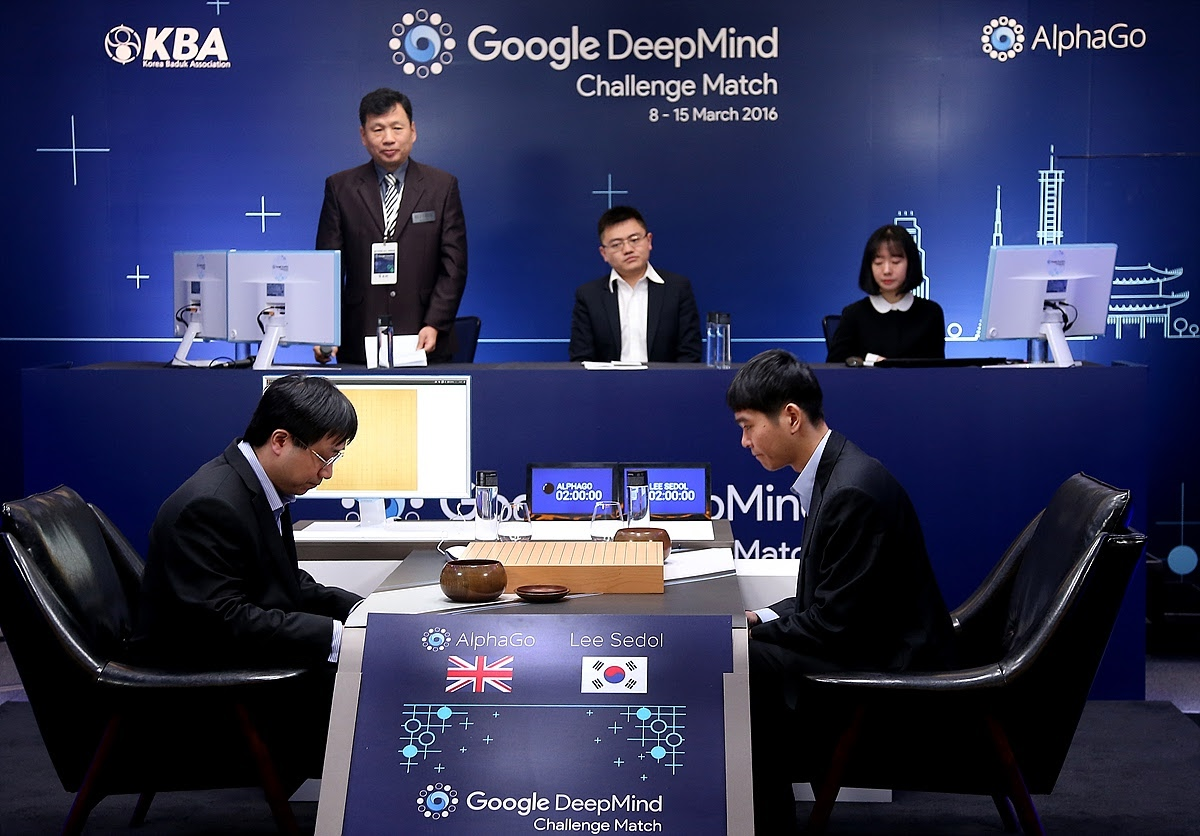
\includegraphics[width=\textwidth]{../images/alpha_go.jpg}
    \end{columns}

    \vspace{0.2cm}
    {\tiny source: DeepMind, AlphaGo research project.}
\end{frame}



\begin{frame}{Autonomous Drone Racing: Beating Human Champions}
    \begin{columns}[T]
        \column{0.56\textwidth}
        \begin{itemize}
            \item deep reinforcement learning system learned
                  to race a physical drone through gates.
            \item in head-to-head races, it won \textbf{15 out of 25}
                  against three champion-level human pilots.
            \item its fastest race was \textbf{0.5 seconds faster}
                  than the best human race time in the study.
        \end{itemize}

        \vspace{0.3cm}
        \textbf{Why it matters:}
        RL can learn fast, reactive control in the physical world,
        not just in games or simulations.

        \column{0.40\textwidth}
        \centering
        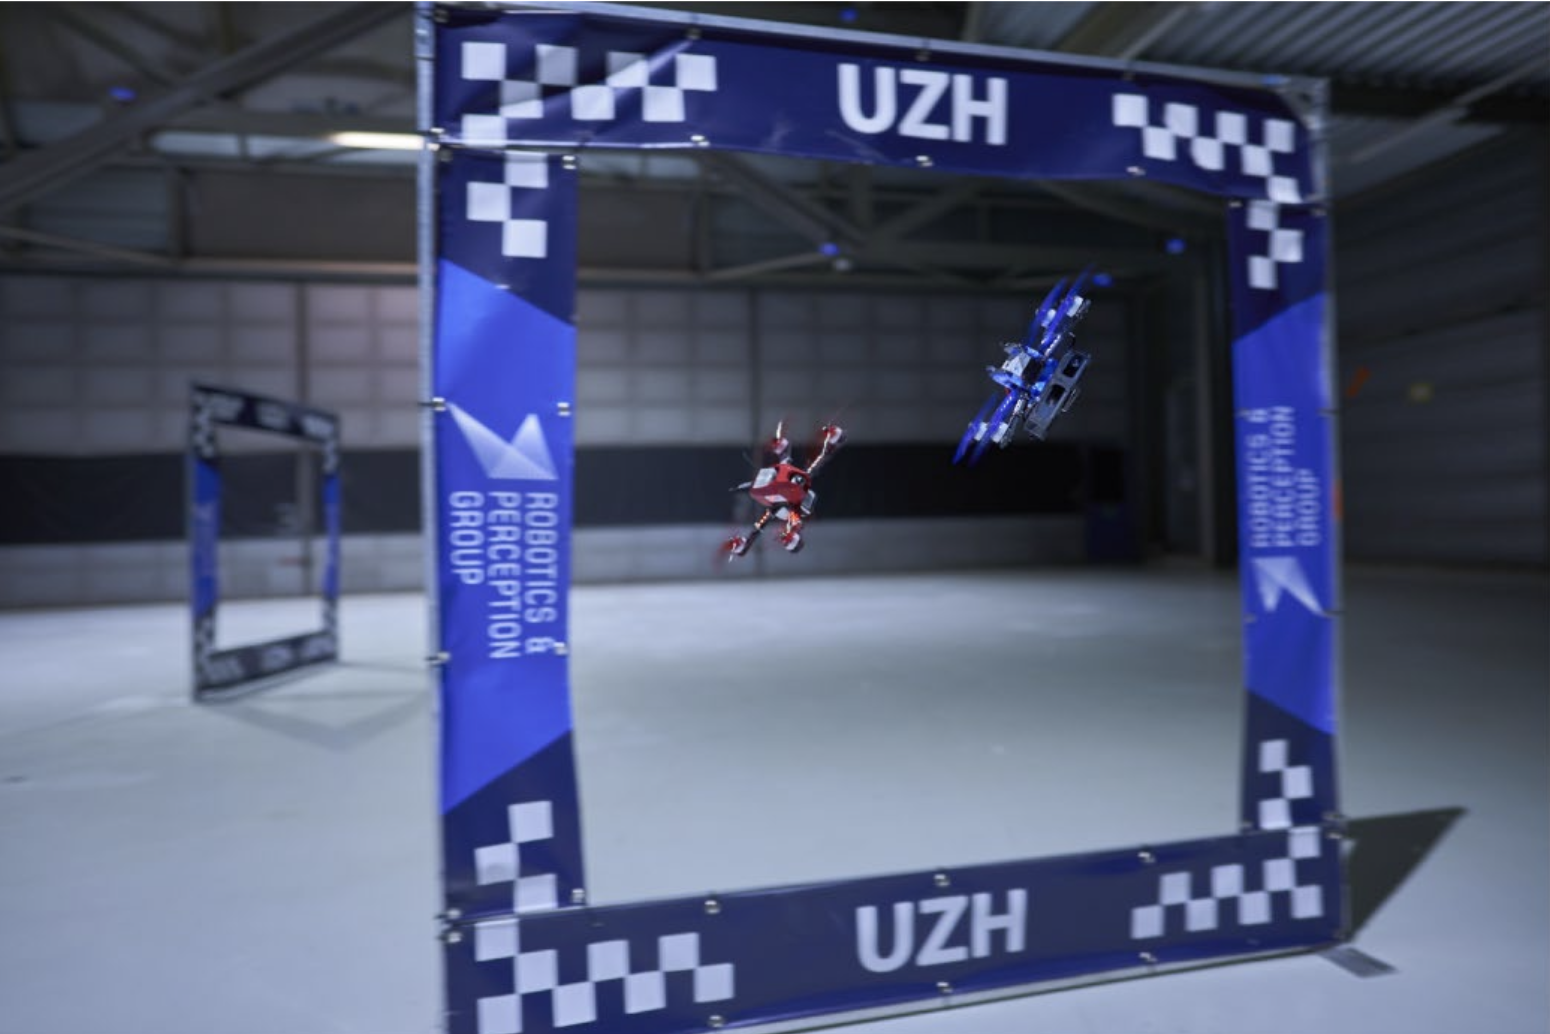
\includegraphics[width=\textwidth]{../images/eth_drone.png}
    \end{columns}

    \vspace{0.2cm}
    {\tiny source: Kaufmann et al., Nature, 2023,
    ``Champion-level drone racing using deep reinforcement learning''.}
\end{frame}




\begin{frame}{\bf Reinforcement learning - principle}

  \centering{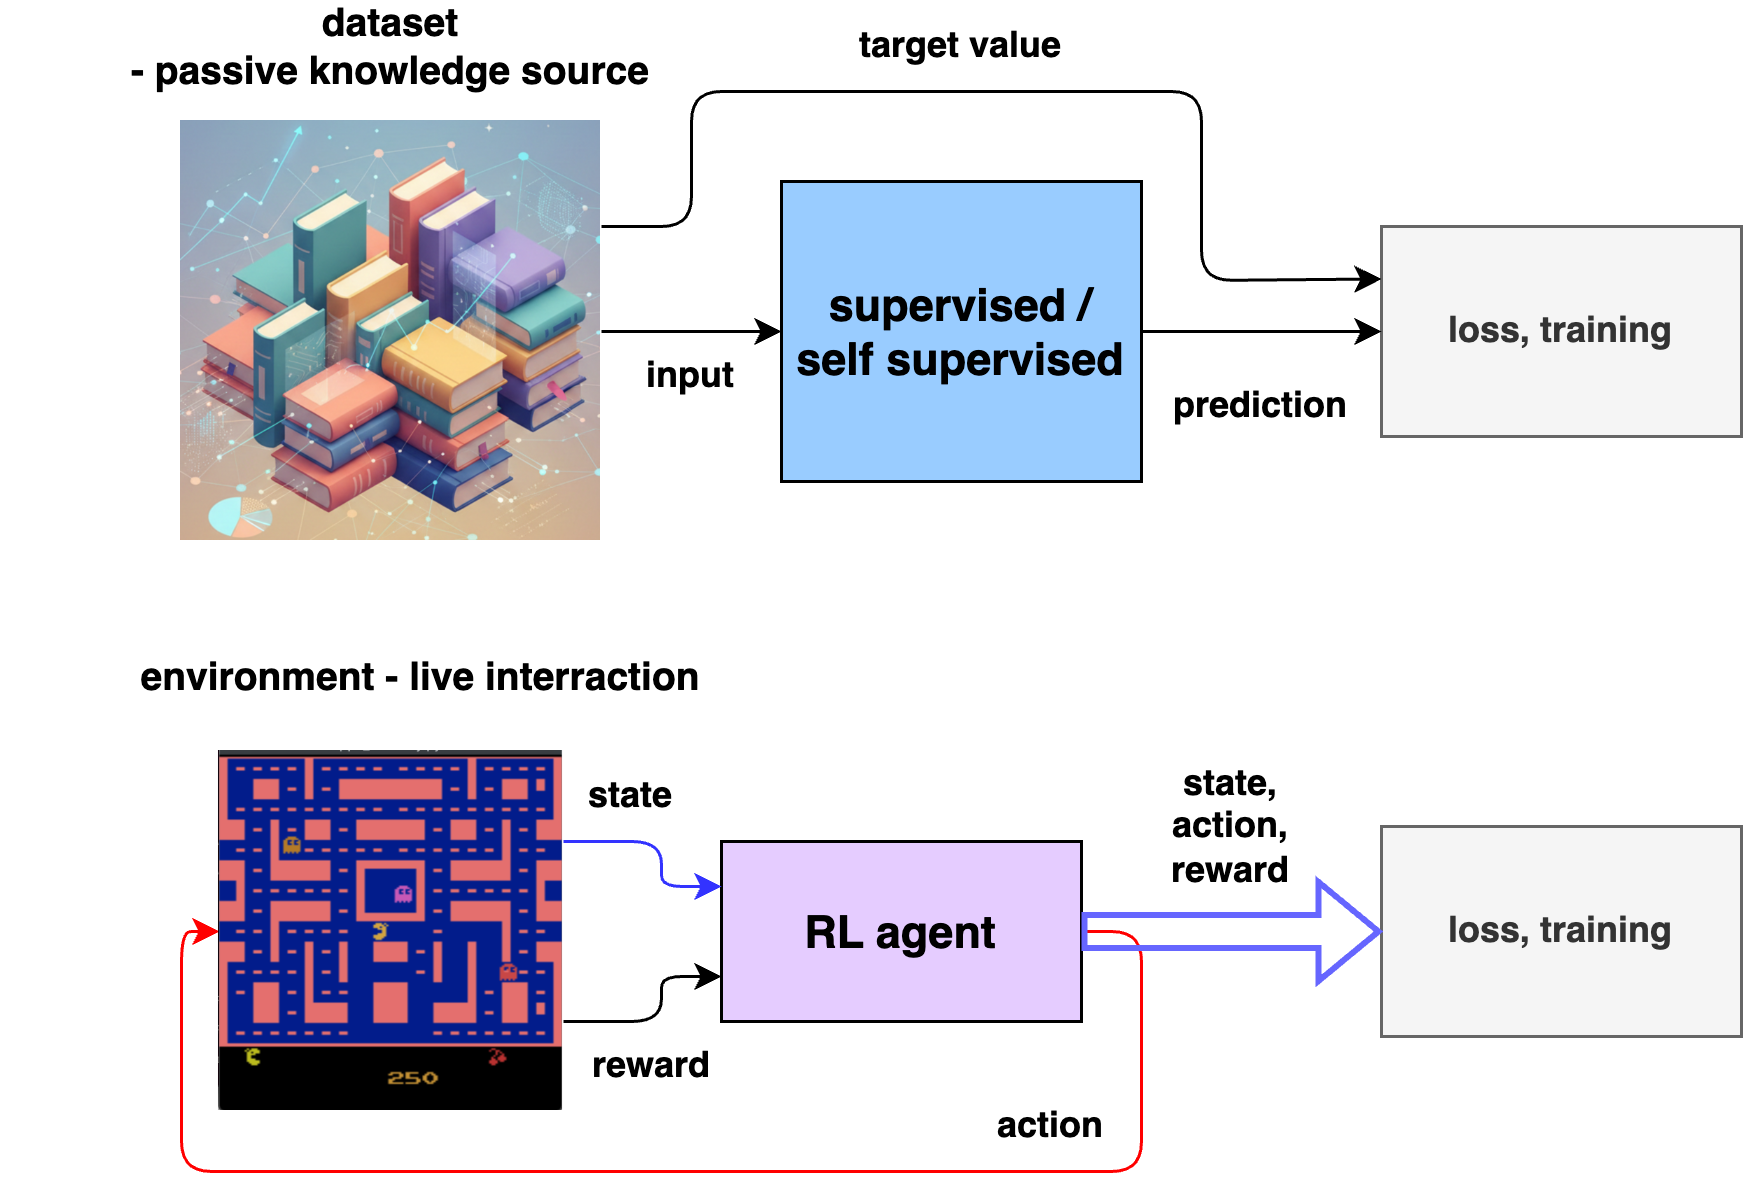
\includegraphics[scale=0.8]{../rl_diagrams/rl_common-comparison.png}}
   
\end{frame}


\begin{frame}{\bf Reinforcement learning - principle}

  \begin{columns}

    \begin{column}{0.5\textwidth}
      \centering{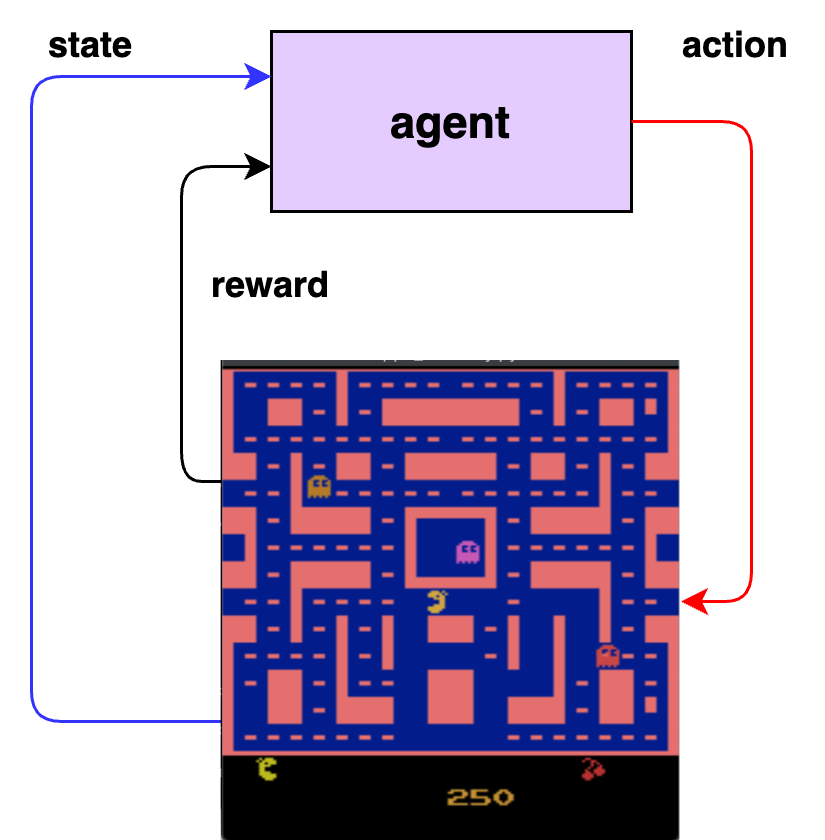
\includegraphics[scale=0.8]{../rl_diagrams/rl_common-principle.png}}
    \end{column}

    \begin{column}{0.5\textwidth}
      \begin{itemize}
        \item \textbf{\textcolor{red}{active environment interraction}}
        \item obtain state
        \item select action
        \item exectute action
        \item learn from experiences
      \end{itemize}
    \end{column}

  \end{columns}

\end{frame}



\begin{frame}{\bf Action space}

  \begin{itemize}
    \item discrete action space \\
      - keys, keypad
    \item continuous action space \\
      - motors, PWMs, steering, torque control
  \end{itemize}

  \centering{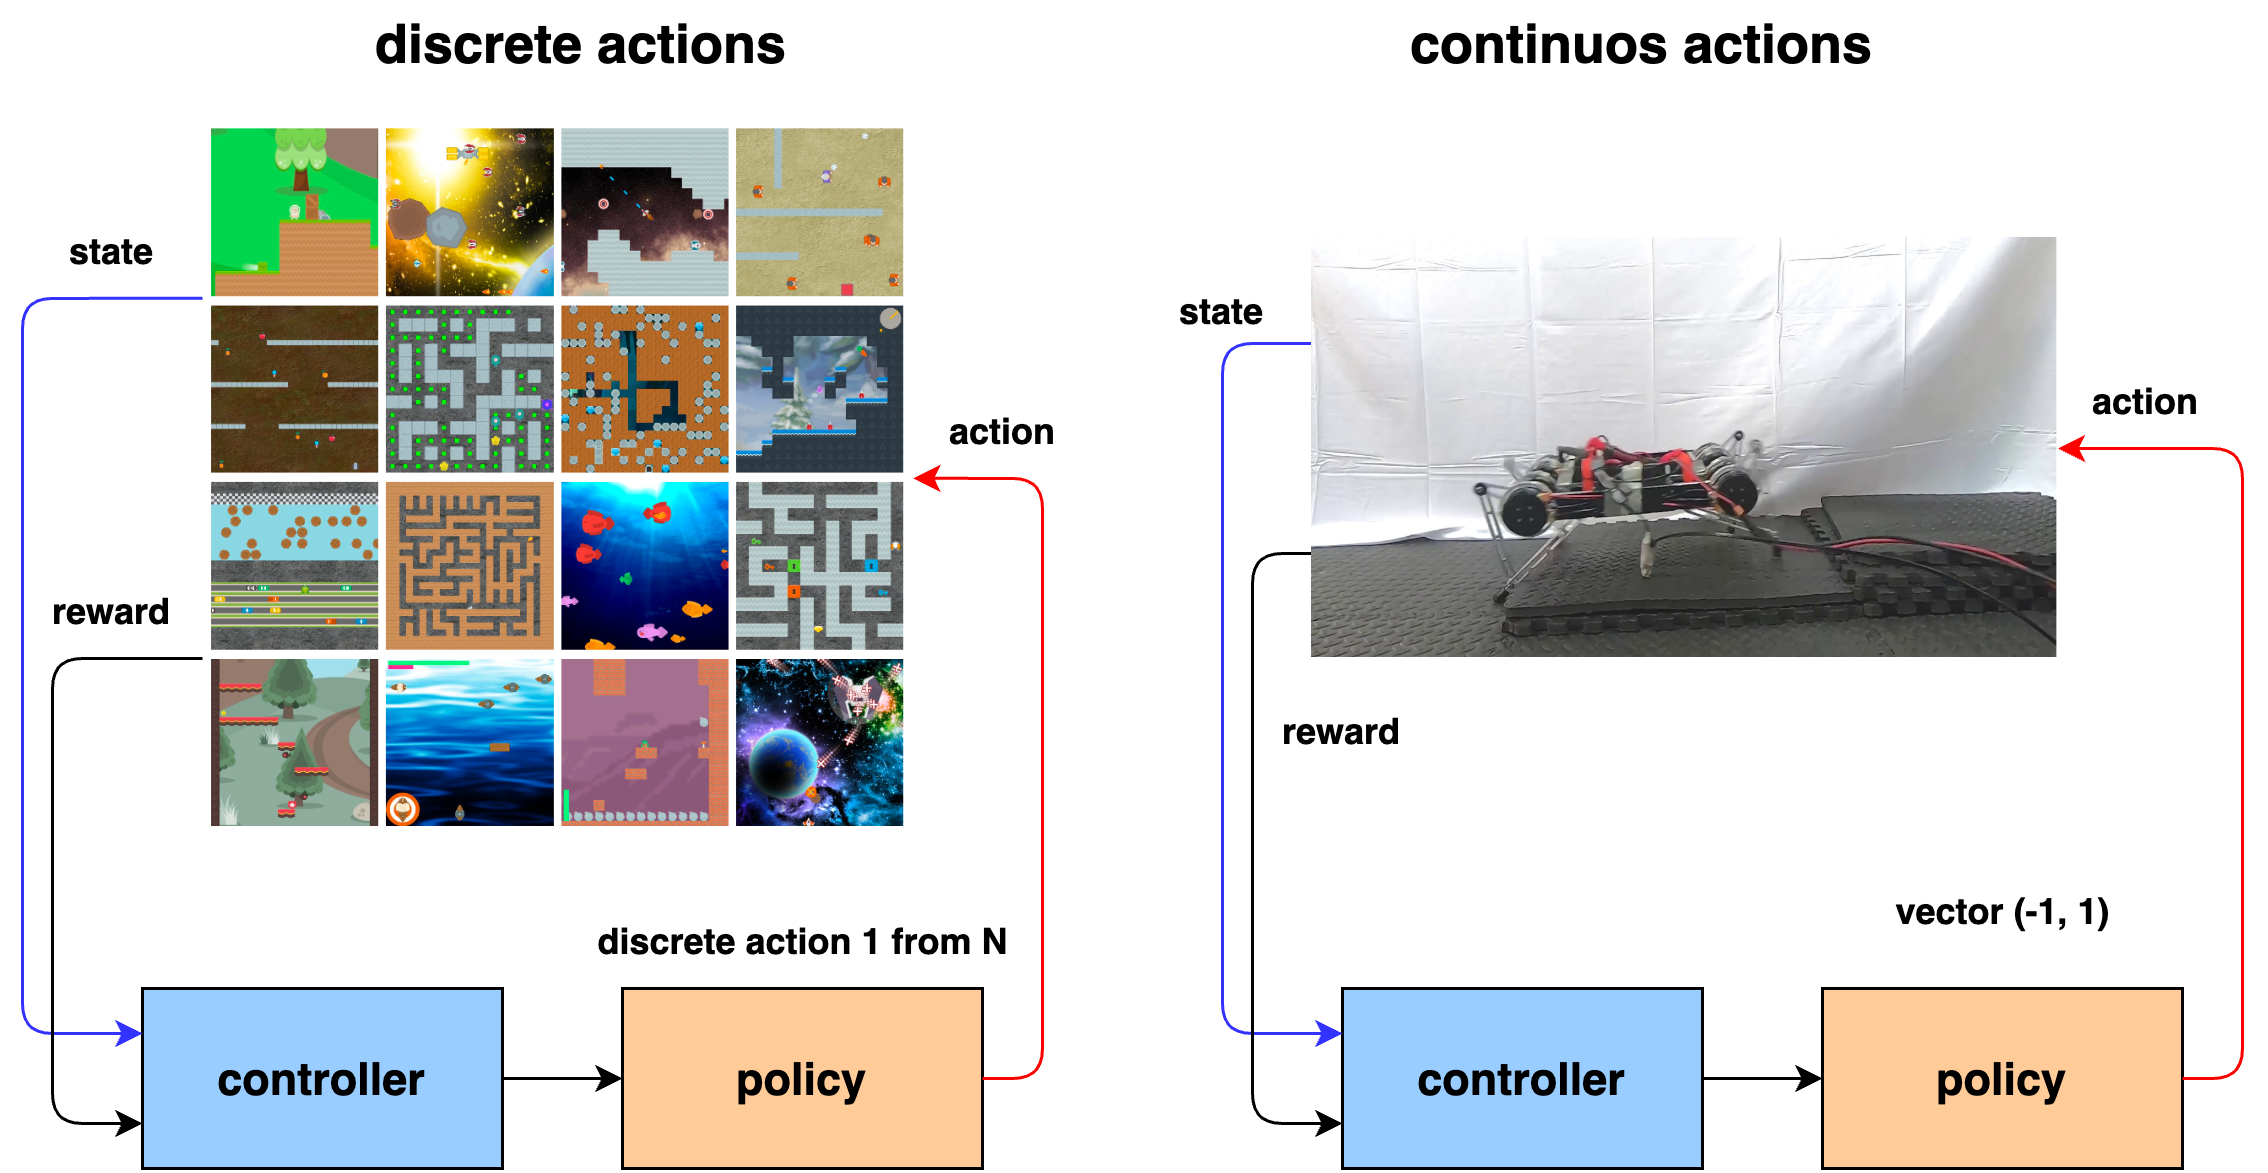
\includegraphics[scale=0.5]{../rl_diagrams/rl_common-actions.png}}

\end{frame}



\begin{frame}{\bf Reinforcement learning - training}

  \centering{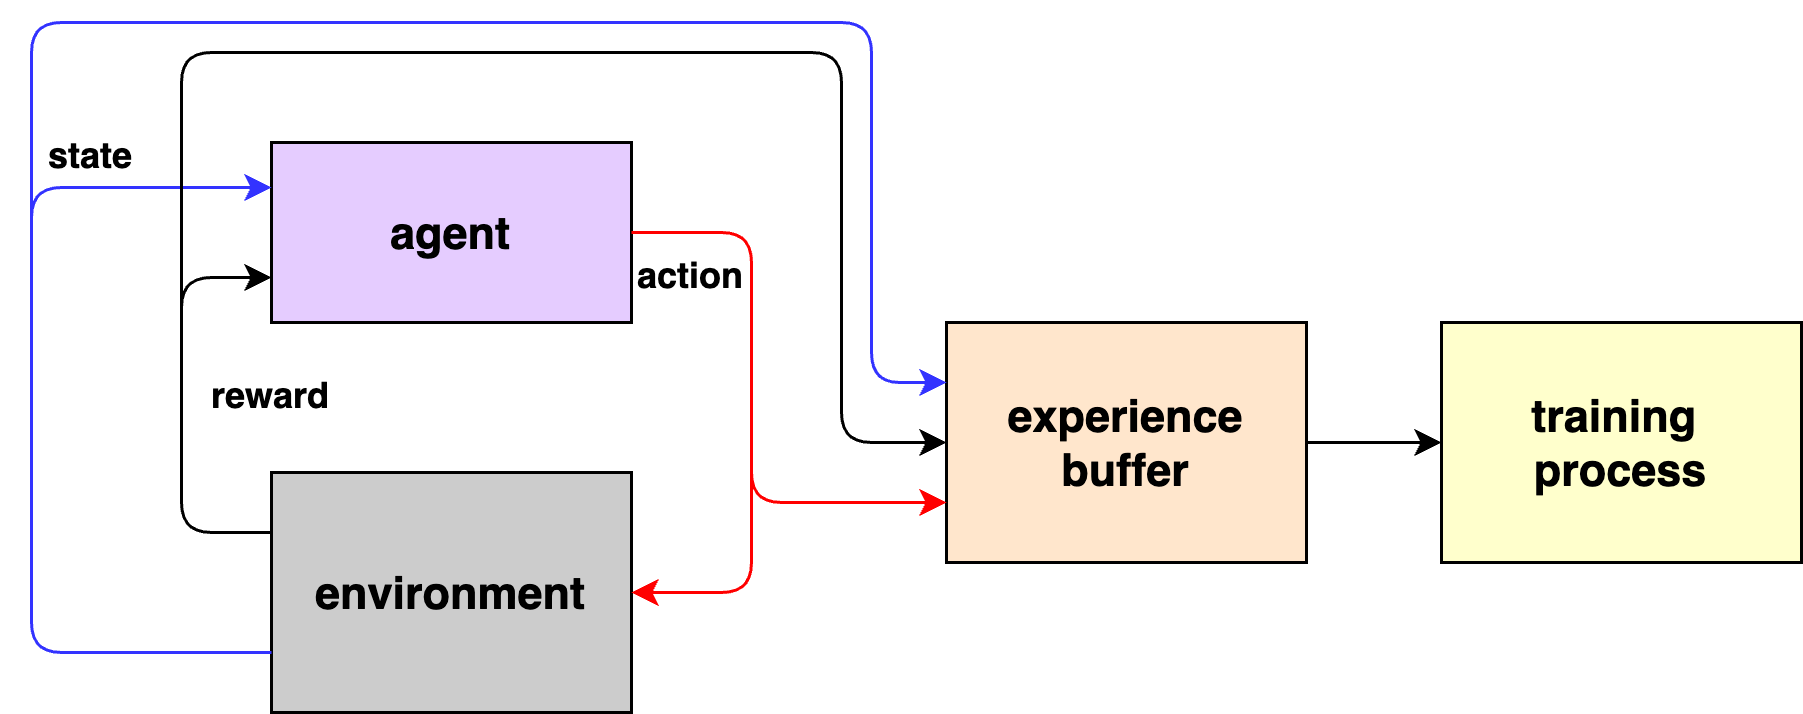
\includegraphics[scale=0.75]{../rl_diagrams/rl_common-training_principle.png}}

  \begin{itemize}
    \item obtain state
    \item select action
    \item exectute action
    \item learn from experiences
  \end{itemize}

\end{frame}



\begin{frame}{\bf Common RL algorithms in practice}

  \small
  \begin{tabular}{p{1.5cm} p{0.8cm} p{2.5cm} p{3.8cm}}
    \hline
    \textbf{algorithm} & \textbf{year} &
    \textbf{best suited for} & \textbf{example / strength}\\
    \hline
    DQN & 2015 &
    discrete actions &
    Atari games; learns values from replayed experience\\[0.15cm]

    A2C / A3C & 2016 &
    discrete or continuous actions &
    Atari and control; intuitive actor--critic baseline\\[0.15cm]

    PPO & 2017 &
    general-purpose policy learning &
    Robotics, locomotion and games; simple, robust baseline\\[0.15cm]

    SAC & 2018 &
    continuous control &
    Robot locomotion and manipulation; sample-efficient\\[0.15cm]

    TD3 & 2018 &
    continuous control &
    MuJoCo locomotion; deterministic actor--critic\\
    \hline
  \end{tabular}

  \vspace{0.3cm}
  \footnotesize
  other important families: REINFORCE (1992), TRPO (2015),
  IMPALA (2018)

\end{frame}




\begin{frame}{\bf Example problem - drone racing}

\centering{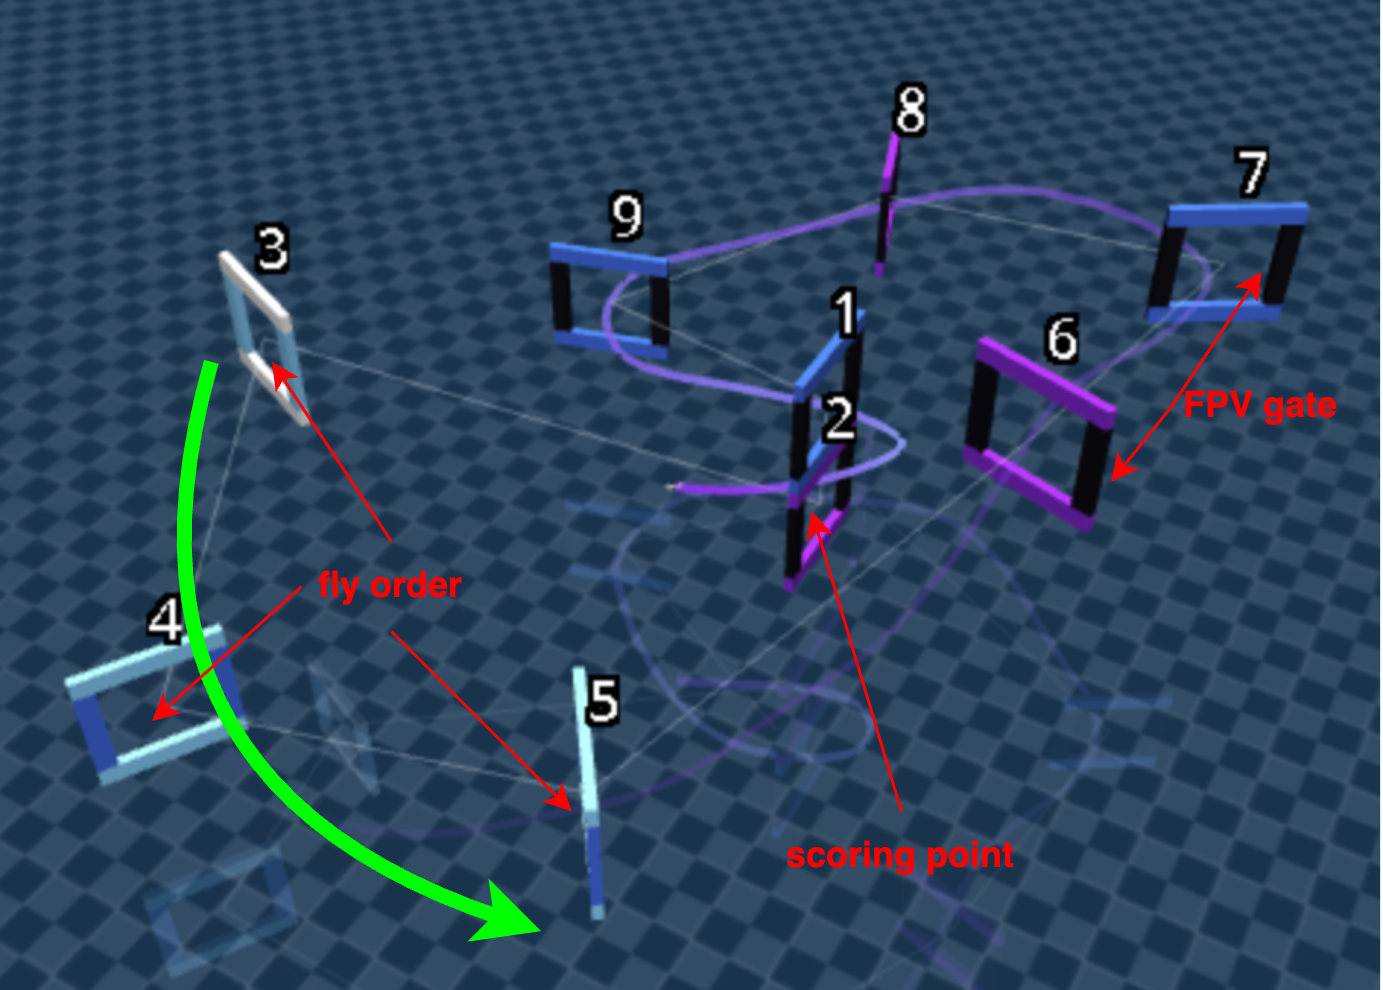
\includegraphics[scale=0.9]{../rl_diagrams/drone_example-environment.png}}

\end{frame}



\begin{frame}{\bf Example problem - drone racing}

  \begin{columns}[T]

    \begin{column}{0.56\textwidth}
      \begin{enumerate}
        \item \textbf{environment design}
        \begin{itemize}
          \item MuJoCo physics simulation
          \item drone, gates and collisions
        \end{itemize}

        \item \textbf{state engineering}
        \begin{itemize}
          \item what does the drone observe?
        \end{itemize}

        \item \textbf{reward engineering}
        \begin{itemize}
          \item how do we define successful flight?
        \end{itemize}

        \item \textbf{agent selection}
        \begin{itemize}
          \item PPO for continuous motor control
        \end{itemize}

        \item \textbf{training and evaluation}
        \begin{itemize}
          \item learn, test and measure performance
        \end{itemize}
      \end{enumerate}
    \end{column}

    \begin{column}{0.42\textwidth}
      \centering
      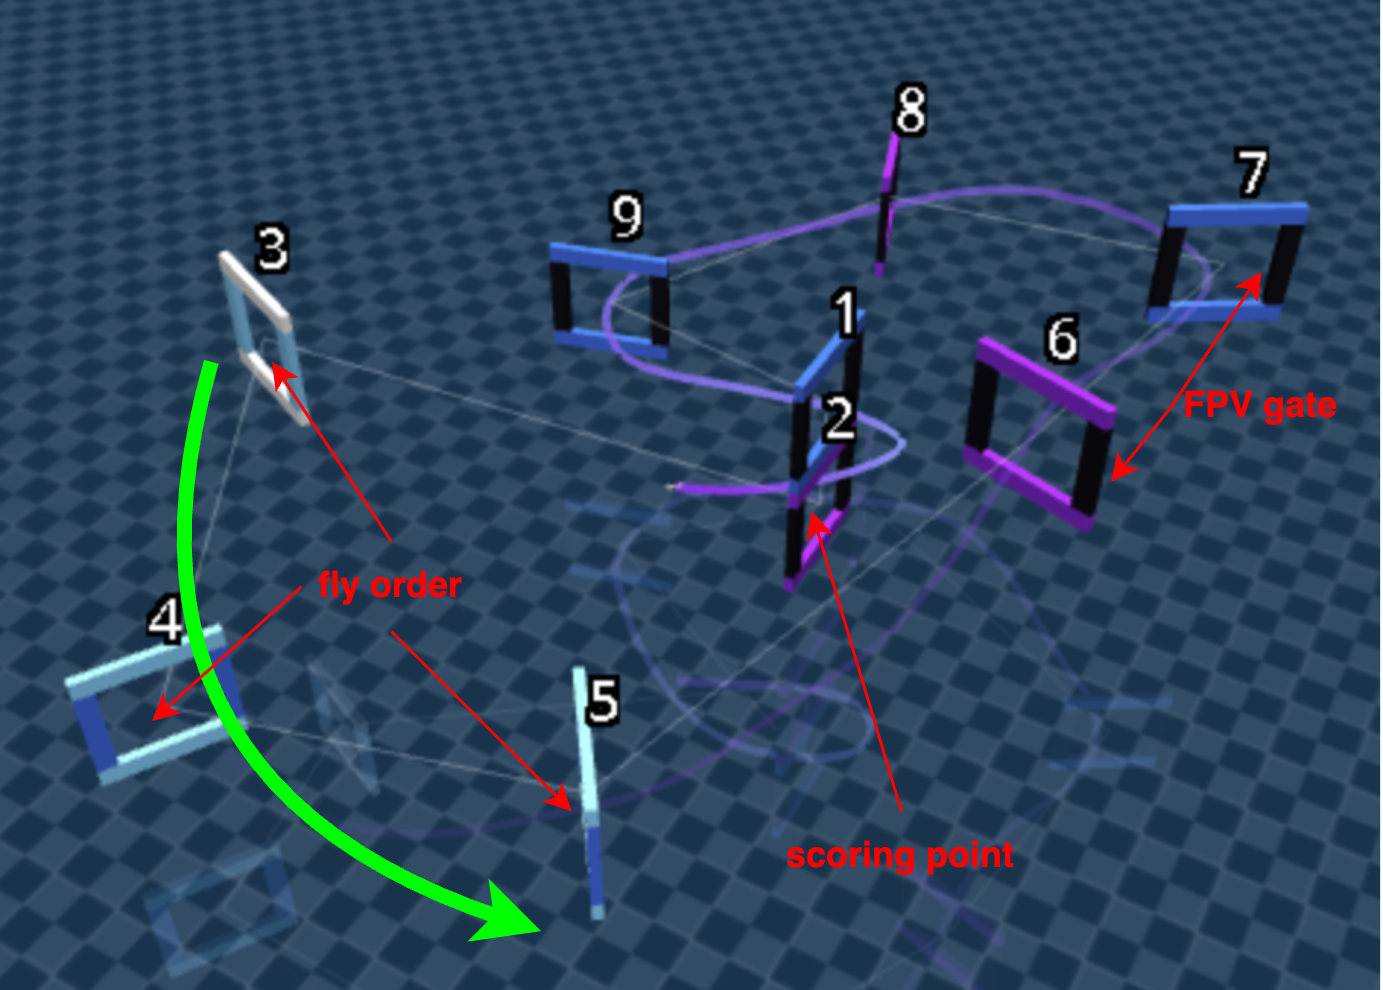
\includegraphics[width=\linewidth]{../rl_diagrams/drone_example-environment.png}
      \vspace{0.3cm}
      \small
      \textcolor{cyan}{fly through the gates in order}
    \end{column}

  \end{columns}

\end{frame}


\begin{frame}{\bf Environment design}

  \begin{columns}[T]

    \begin{column}{0.55\textwidth}
      \centering
      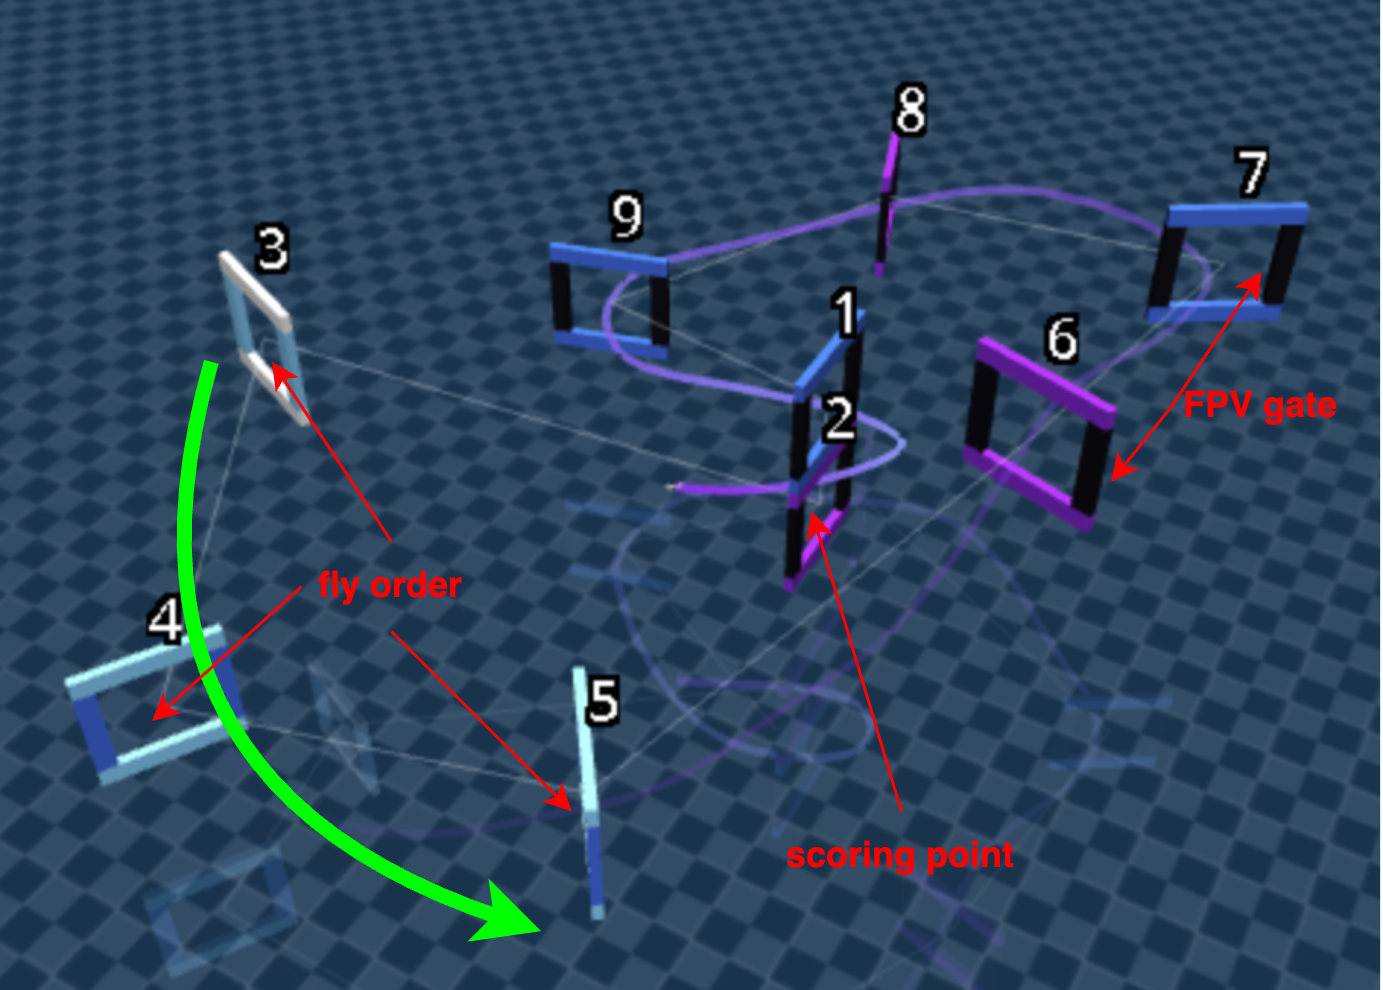
\includegraphics[width=\linewidth]
        {../rl_diagrams/drone_example-environment.png}
    \end{column}

    \begin{column}{0.43\textwidth}
      \textbf{Simulation setup}
      \begin{itemize}
        \item Crazyflie CF2X quadrotor
        \item MuJoCo physics engine
        \item 250 Hz physics simulation
        \item 50 Hz control frequency
        \item 5 physics steps per action
        \item 60 s maximum episode
      \end{itemize}
    \end{column}

  \end{columns}

  \vspace{0.2cm}
  \begin{block}{Task}
    Fly through square gates in the prescribed order.
    Colliding with a gate frame terminates the episode.
  \end{block}

\end{frame}


\begin{frame}{\bf Environment design}
  \centering
  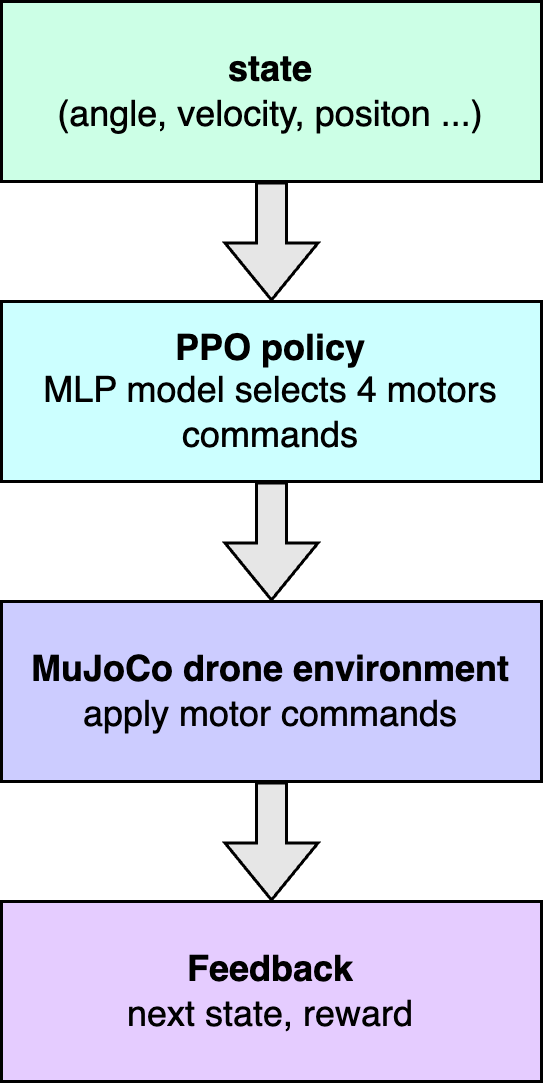
\includegraphics[scale=0.8]{../rl_diagrams/drone_example-env_block.png}
\end{frame}


\begin{frame}{\bf State Engineering}

  \textbf{observation: what does the drone know?}

  \begin{itemize}
    \item \textbf{attitude (4):}
      $\sin(\phi),\cos(\phi),\sin(\theta),\cos(\theta)$
    \item \textbf{angular velocity (3):}
      $\omega_x,\omega_y,\omega_z$
    \item \textbf{linear velocity (2):}
      velocity over ground
    \item \textbf{height (2):}
      distance above the floor and velocity
    \item \textbf{upcoming gates (36):}
      four 3D inner corners for each of three gates
    \item \textbf{nearest gate (12):}
      collision avoidance 
  \end{itemize}

  \begin{block}{observation vector}
    \[
      s_t \in \mathbb{R}^{59},
      \qquad 11 + 3\cdot 12 + 12 = 59
    \]
    the observation is drone-centric: no absolute world
    position or world yaw is provided. 
  \end{block}


\end{frame}


\begin{frame}{\bf State Engineering - why these features?}

  \begin{itemize}
    \item \textbf{attitude and angular velocity}
      \begin{itemize}
        \item stabilize the drone and detect rotation.
      \end{itemize}

    \item \textbf{velocity and height}
      \begin{itemize}
        \item estimate motion and maintain safe flight.
      \end{itemize}

    \item \textbf{relative gate geometry}
      \begin{itemize}
        \item determine where the gate is and how it is oriented.
        \item plan the approach using upcoming gates.
      \end{itemize}
  \end{itemize}

  \begin{alertblock}{Design principle}
    give the policy task-relevant information in a
    consistent coordinate frame, not arbitrary world
    coordinates.
  \end{alertblock}

\end{frame}




\begin{frame}{\bf Reward Engineering}

  \textbf{goal: pass gates in the correct order without crashing.}

  \begin{itemize}
    \item gate passed: positive reward
    \item progress towards the next gate: shaping reward
    \item better gate alignment: shaping reward
    \item collision or crash: penalty
  \end{itemize}

  \begin{block}{Reward function}
    \[
      r_t =
      \begin{cases}
        R_{\mathrm{gate}}, & \text{if next gate passed},\\
        \Phi(s_t)-\Phi(s_{t-1}), & \text{otherwise}
      \end{cases}
    \]
    \[
      r_t \leftarrow r_t -
      R_{\mathrm{crash}}\,\mathbb{1}_{\mathrm{crash}}
    \]
  \end{block}

  \small
  Default values:
  $R_{\mathrm{gate}}=1$,
  $R_{\mathrm{crash}}=1$.

\end{frame}


\begin{frame}{\bf Reward Engineering - shaping}

  define a potential function:
  \[
    \Phi(s) =
    -k_d d_{\mathrm{gate}}(s)
    + k_a A_{\mathrm{gate}}(s)
  \]

  \begin{itemize}
    \item $d_{\mathrm{gate}}$: distance to the next gate centre
    \item $A_{\mathrm{gate}}$: gate-alignment score
    \item $k_d,k_a$: shaping weights
  \end{itemize}

  \vspace{0.2cm}
  \begin{block}{Key idea}
    \[
      r_t^{\mathrm{shape}} = \Phi(s_t)-\Phi(s_{t-1})
    \]
    reward changes in progress and alignment, rather than
    rewarding their absolute values at every step.
  \end{block}

  \small
  with the potential reset handled consistently at gate
  transitions, this shaping avoids rewarding the agent
  simply for hovering near a gate.

\end{frame}


 


\begin{frame}{\bf Agent selection - PPO}

  \textbf{why PPO?}

  \begin{itemize}
    \item continuous action space: four motor commands
    \item stochastic policy enables exploration
    \item actor-critic architecture learns actions and values
    \item clipped objective limits incentives for large policy changes
  \end{itemize}

  \begin{block}{continuous policy}
    \[
      \pi_\theta(a|s)=
      \mathcal{N}\left(
        \mu_\theta(s),
        \operatorname{diag}(\sigma_\theta^2(s))
      \right)
    \]
    \[
      a_t=\mu_\theta(s_t)+
      \sigma_\theta(s_t)\odot\epsilon,\qquad
      \epsilon\sim\mathcal{N}(0,I)
    \]
  \end{block}

  \small
  the model predicts the action mean, action variance and
  state value. The environment clips motor commands to
  $[-1,1]^4$.

\end{frame}



\begin{frame}{\bf Agent selection - Model}
  \centering
  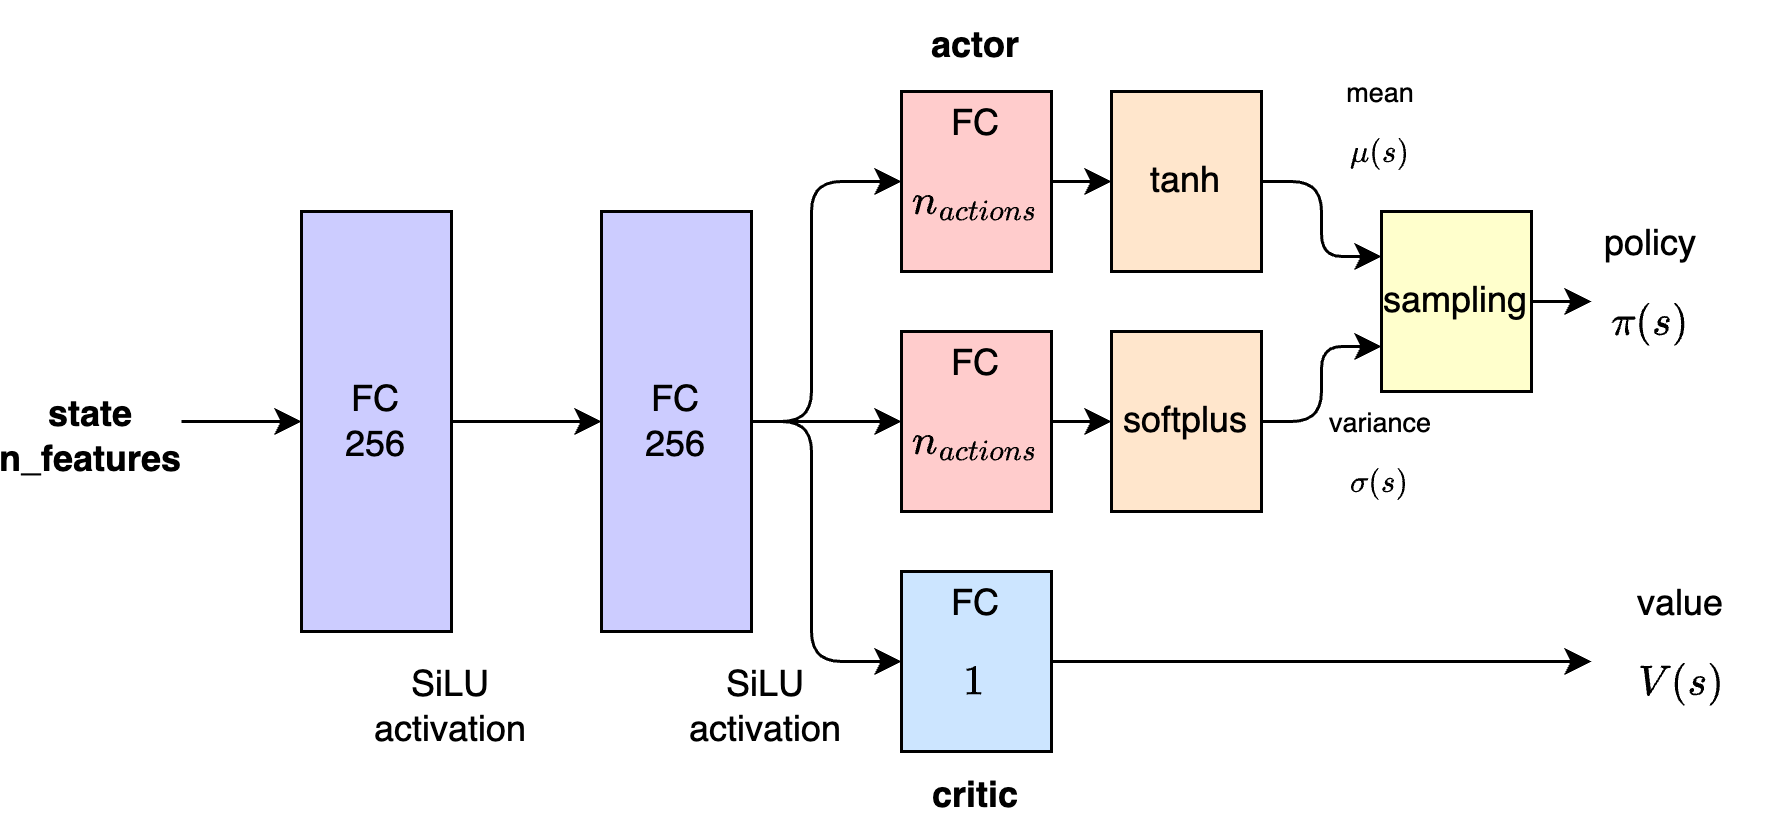
\includegraphics[scale=0.8]{../rl_diagrams/rl_common-mlp_cont_model.png}
\end{frame}


\begin{frame}{\bf PPO - learning from experience}
  \centering
  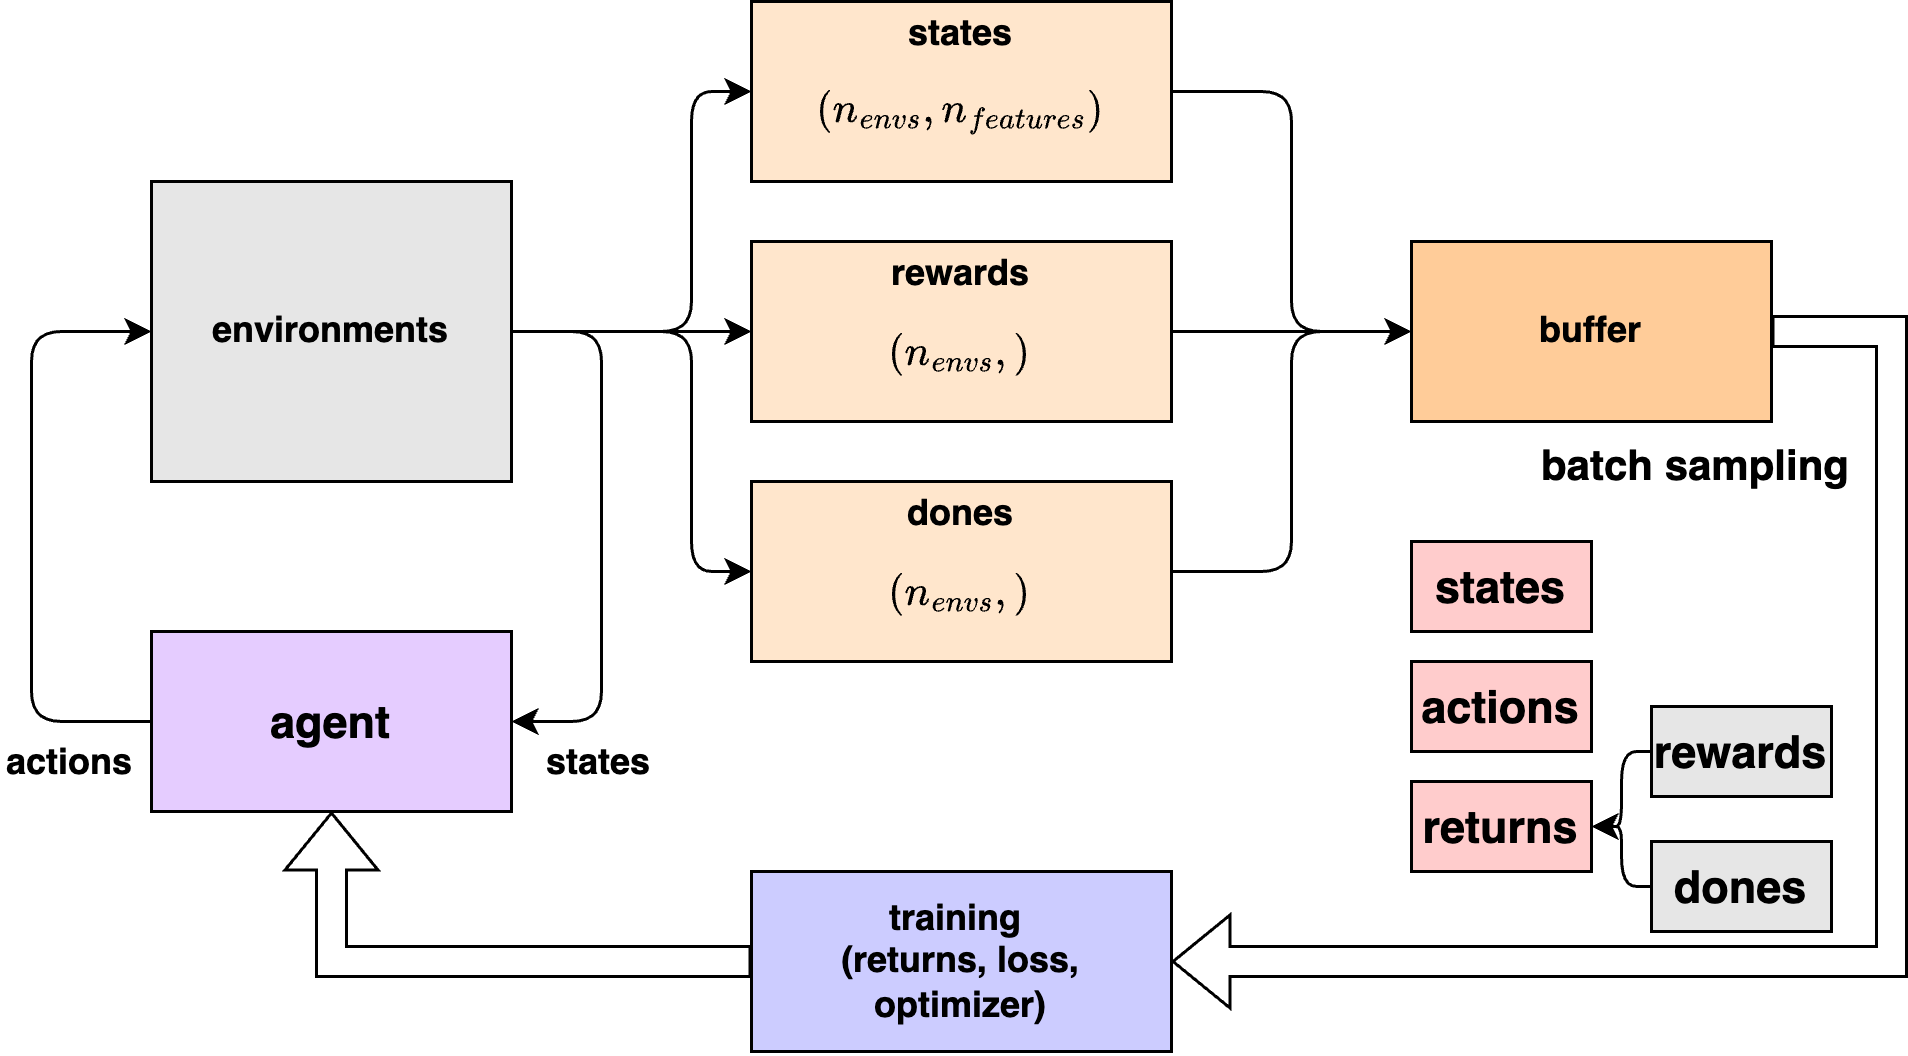
\includegraphics[scale=0.7]{../rl_diagrams/a2c-training_00.png}

\end{frame}




\begin{frame}{\bf Evaluation - does the drone learn to race?}

  \textbf{evaluation of the policy}

  \begin{itemize}
    \item \textbf{episodic  score}
    \item \textbf{gates passed:} mean number of successful crossings
    \item \textbf{flight speed and g-force:} mean and maximum speed
    \item \textbf{completion ratio:} gates passed / gates in course
    \item \textbf{crash rate:} fraction of episodes ending in a crash
    \item \textbf{generalization:} performance on unseen gate layouts
  \end{itemize}


\end{frame}



\begin{frame}{\bf Passed gates}
  \centering
  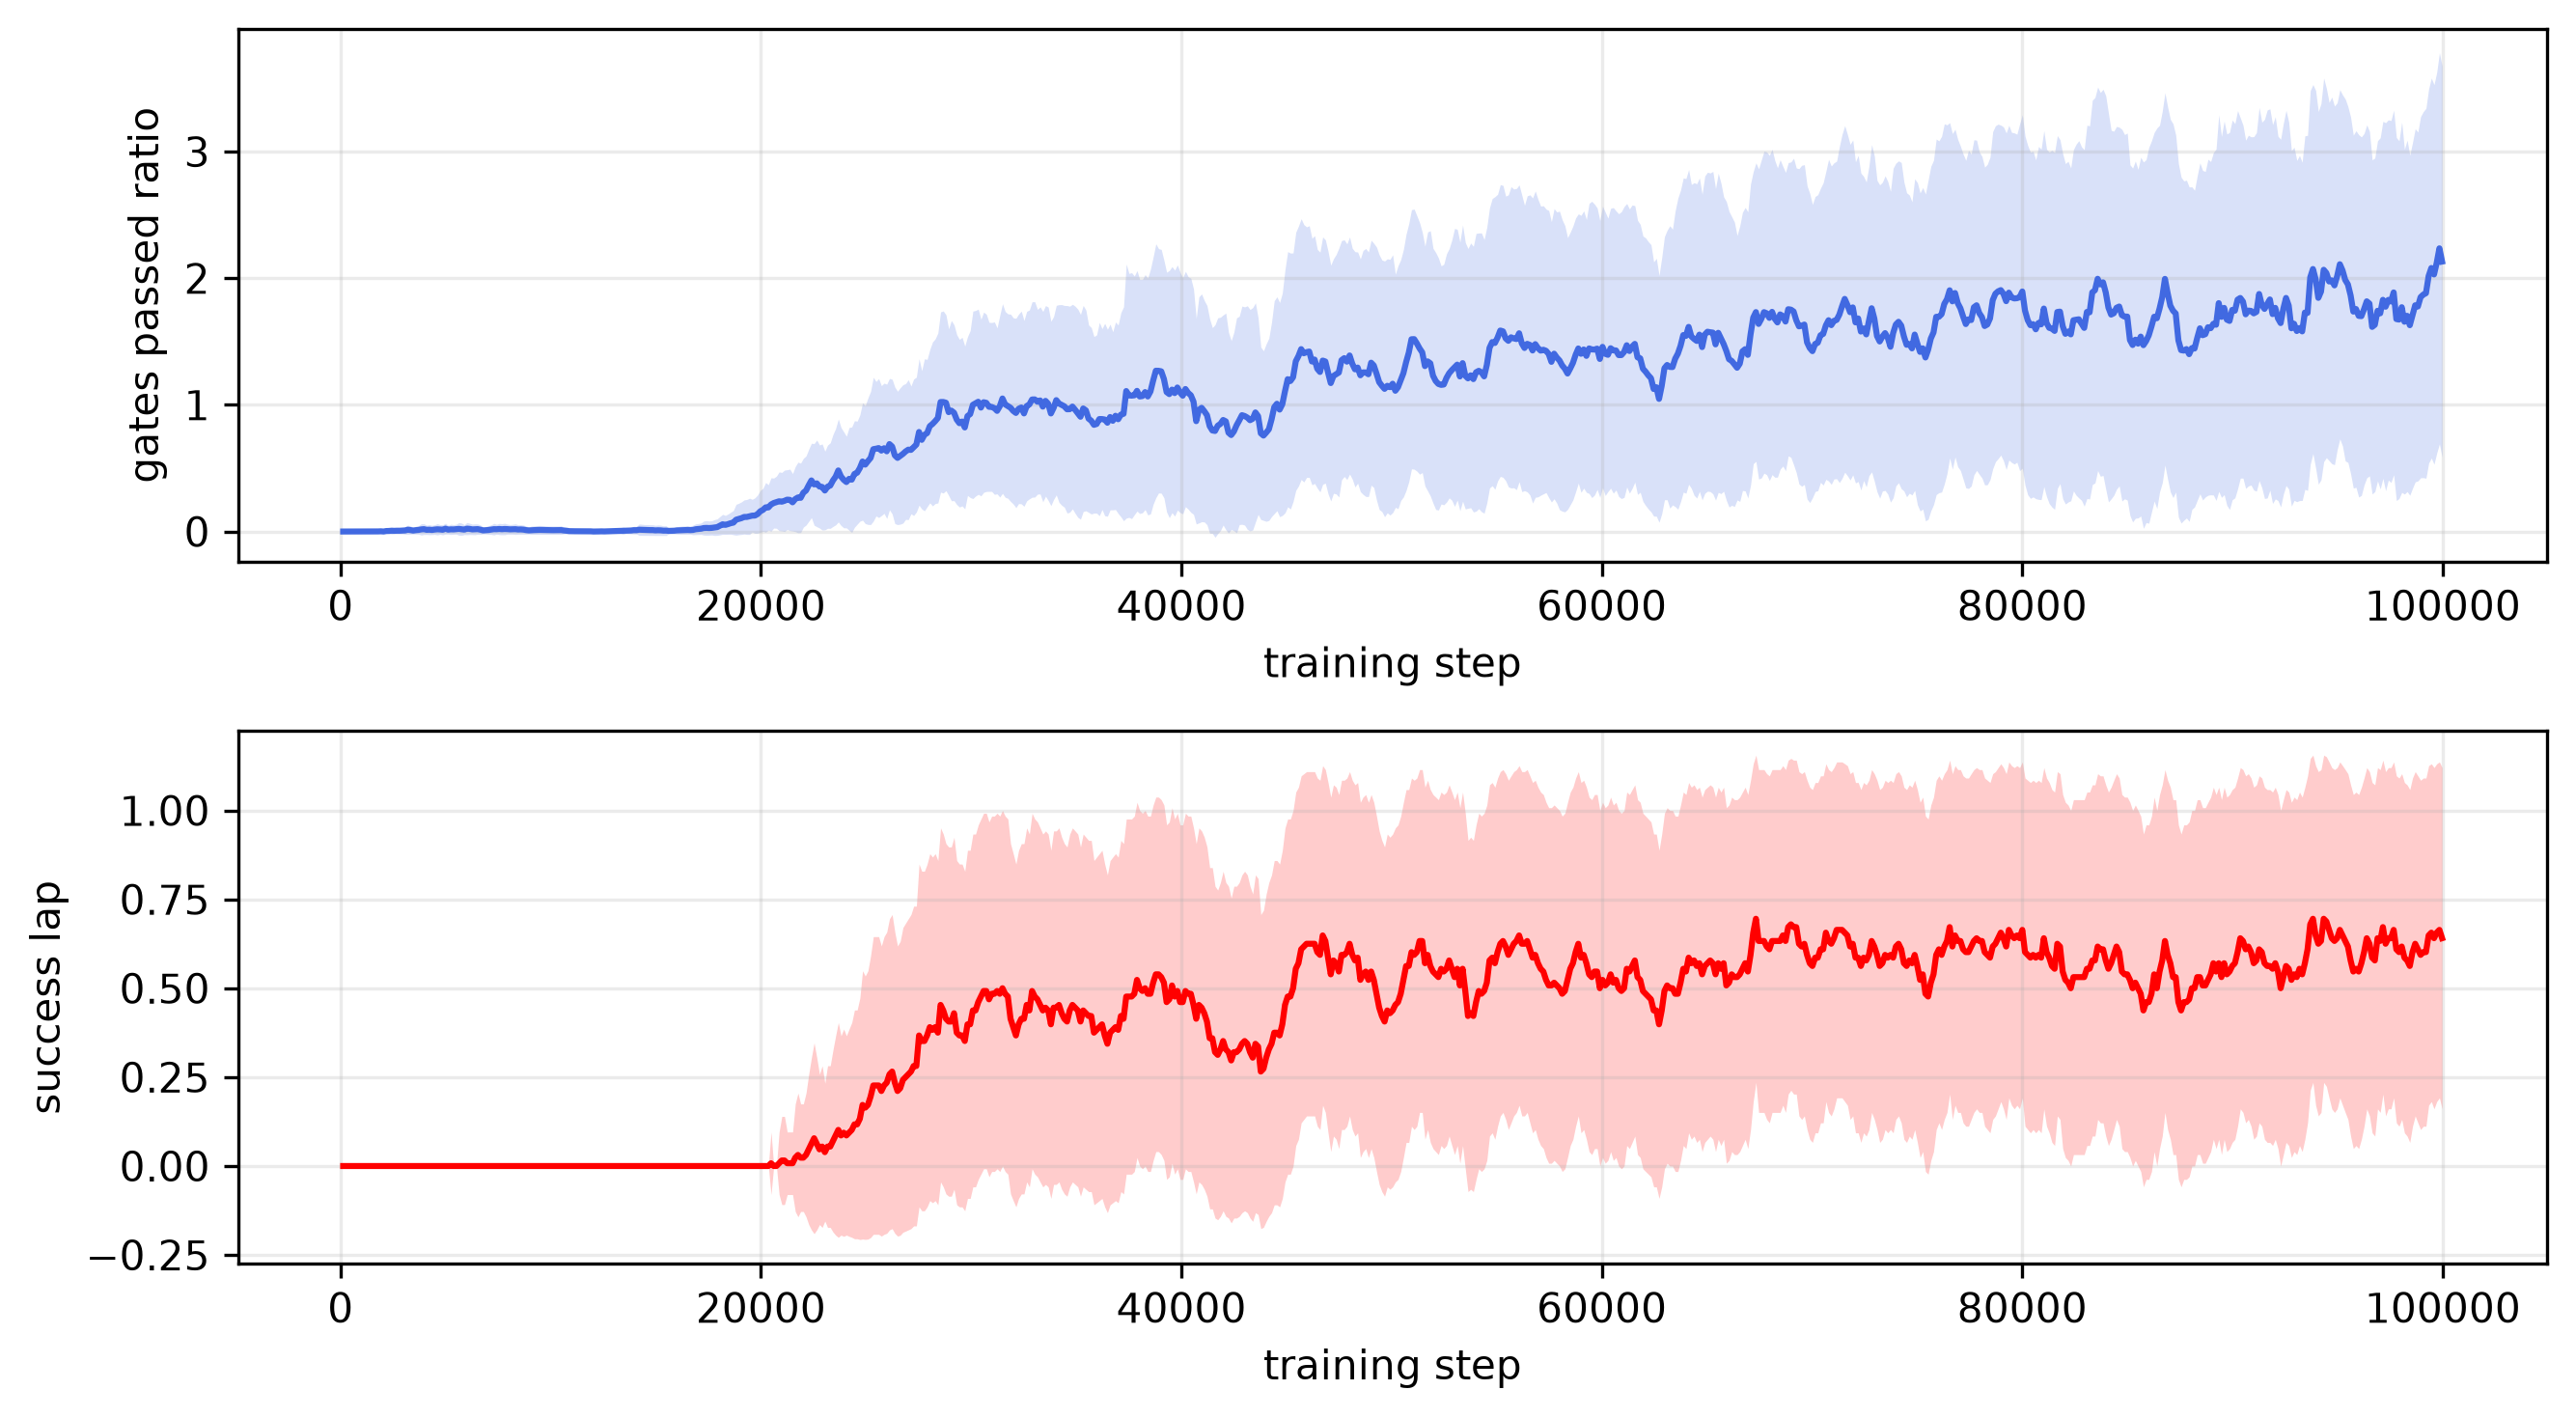
\includegraphics[scale=0.5]{../rl_drones_results/env_success_rate.png}

\end{frame}


\begin{frame}{\bf Speed and forces}
  \centering
  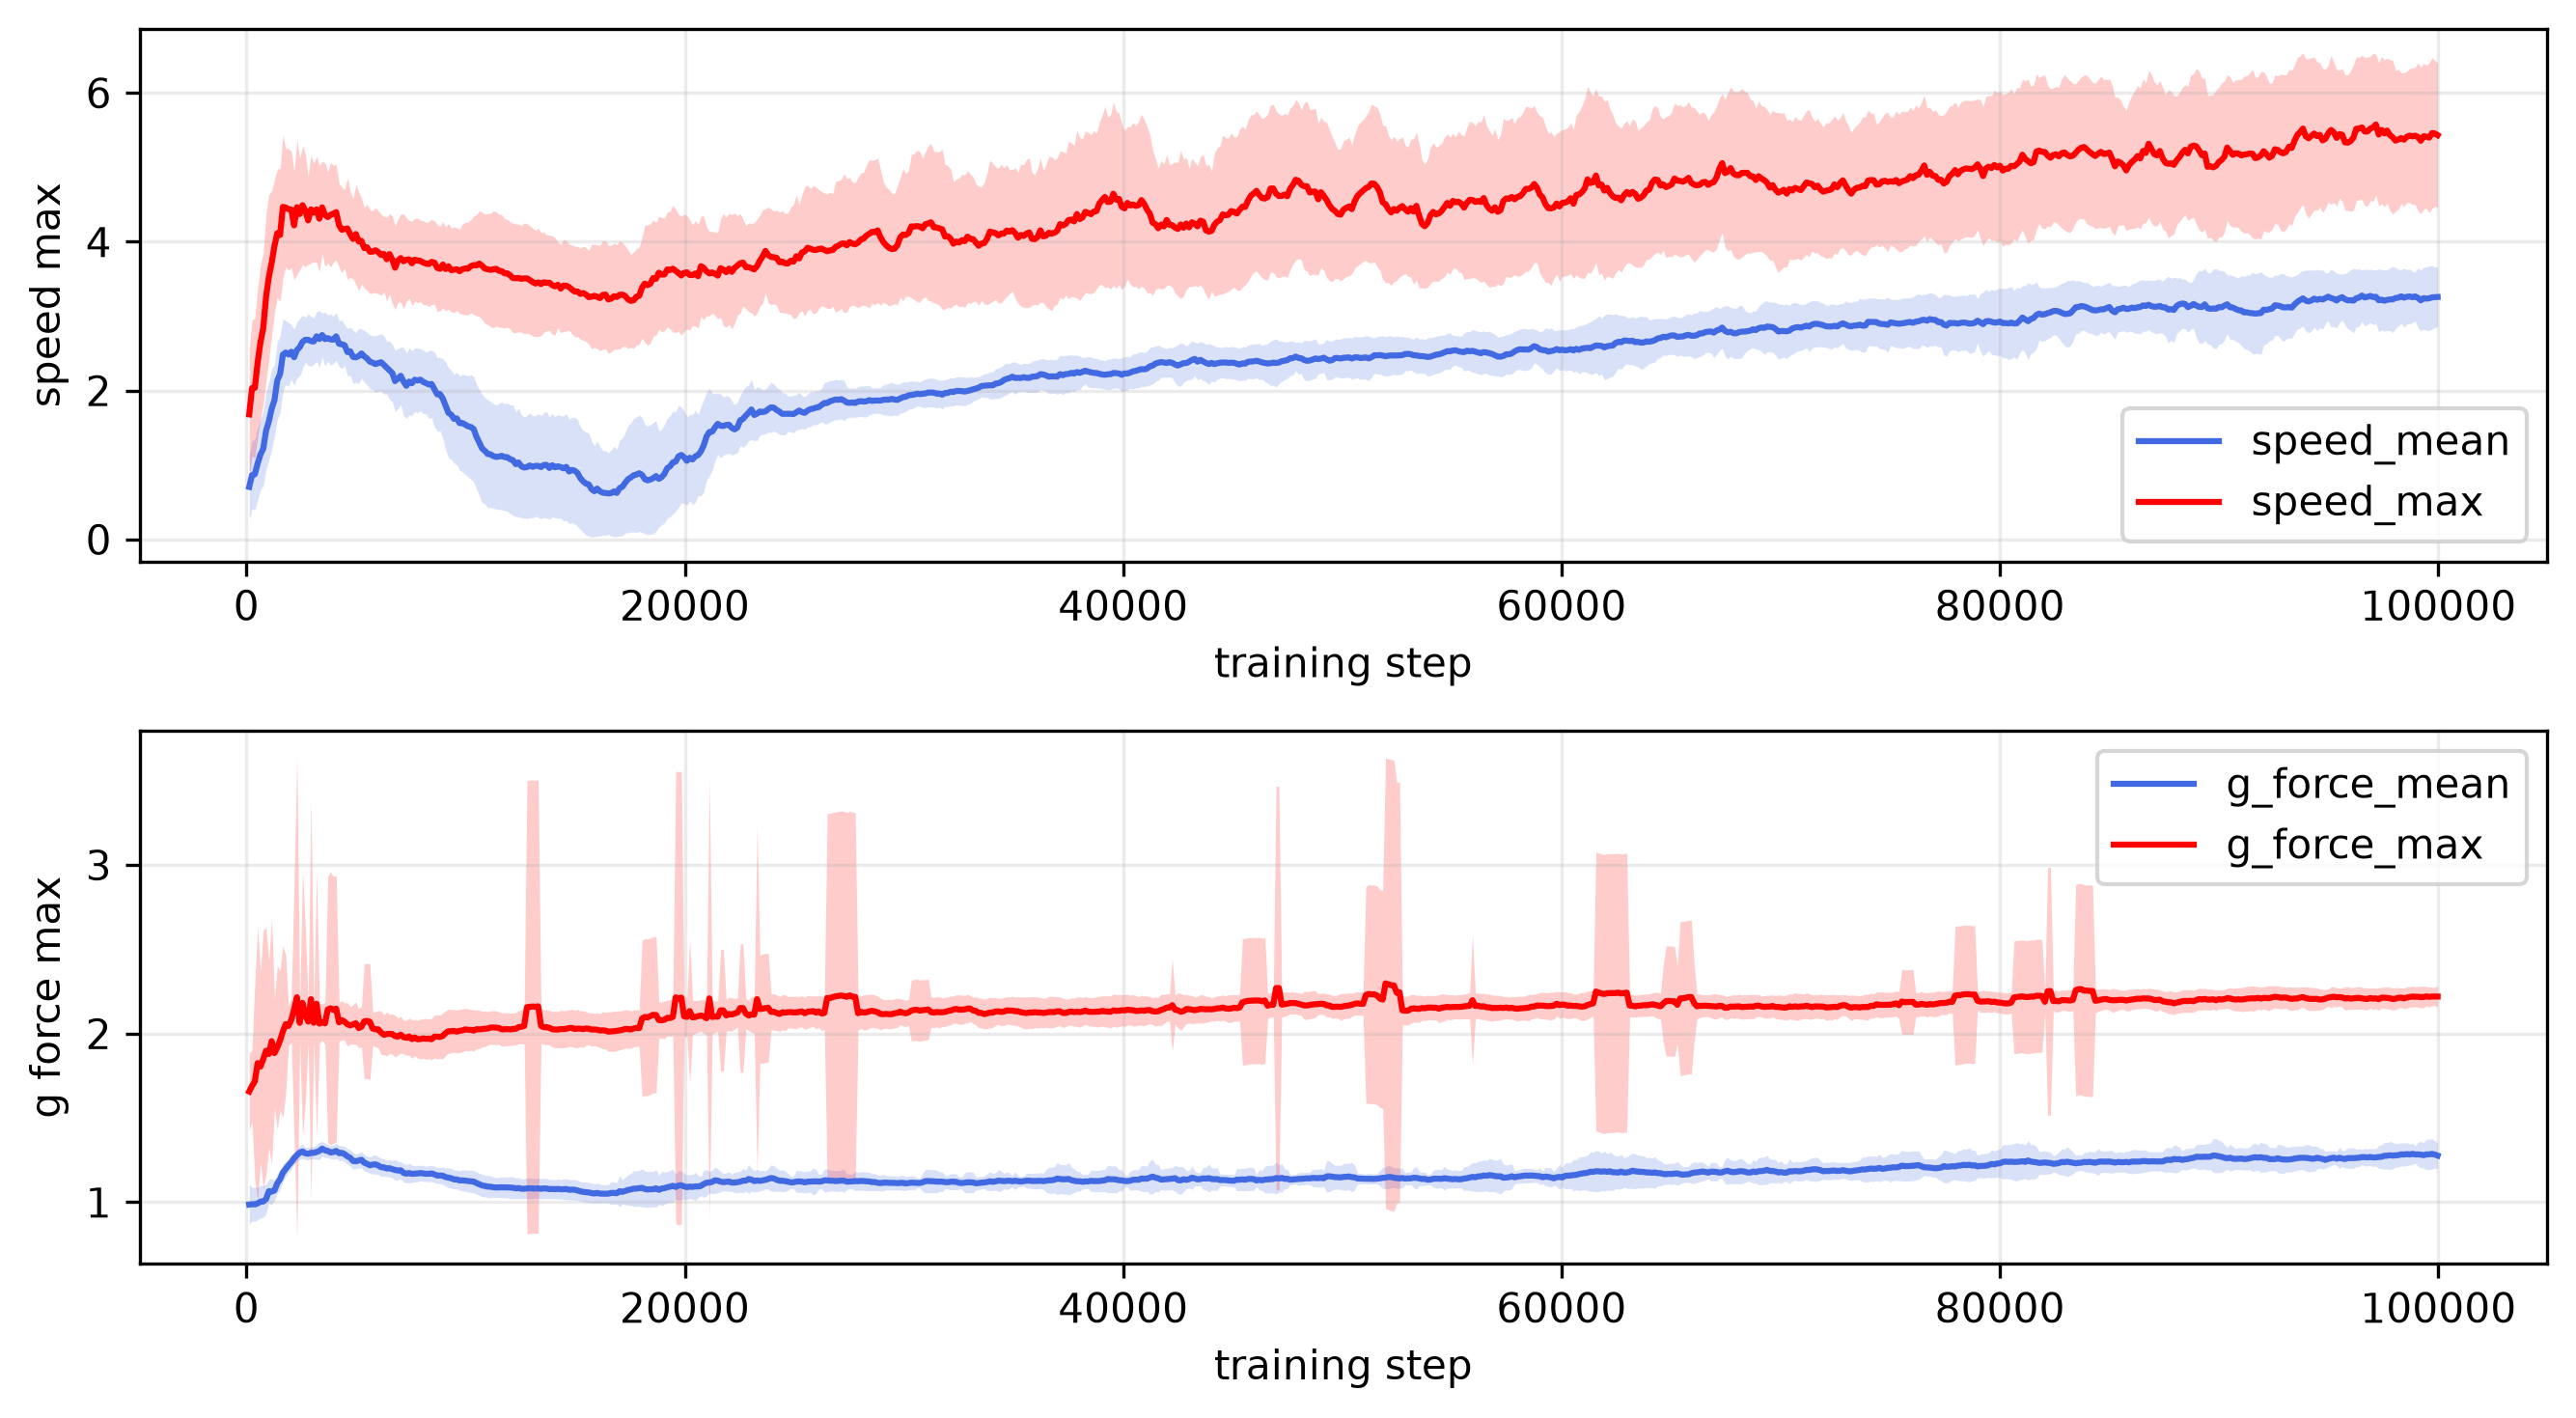
\includegraphics[scale=0.5]{../rl_drones_results/env_speed_force.png}
\end{frame}

\begin{frame}{\bf Policy Gradients, Advantage-Actor-Critic (A2C)}

  \begin{itemize}
    \item \textbf{actor:} selects an action using policy
      $\pi_\theta(a|s)$
    \item \textbf{critic:} estimates expected future return
      $V_\phi(s)$
    \item \textbf{advantage:} tells the actor whether an
      action was better than expected
  \end{itemize}

  \vspace{0.1cm}
  \centering
  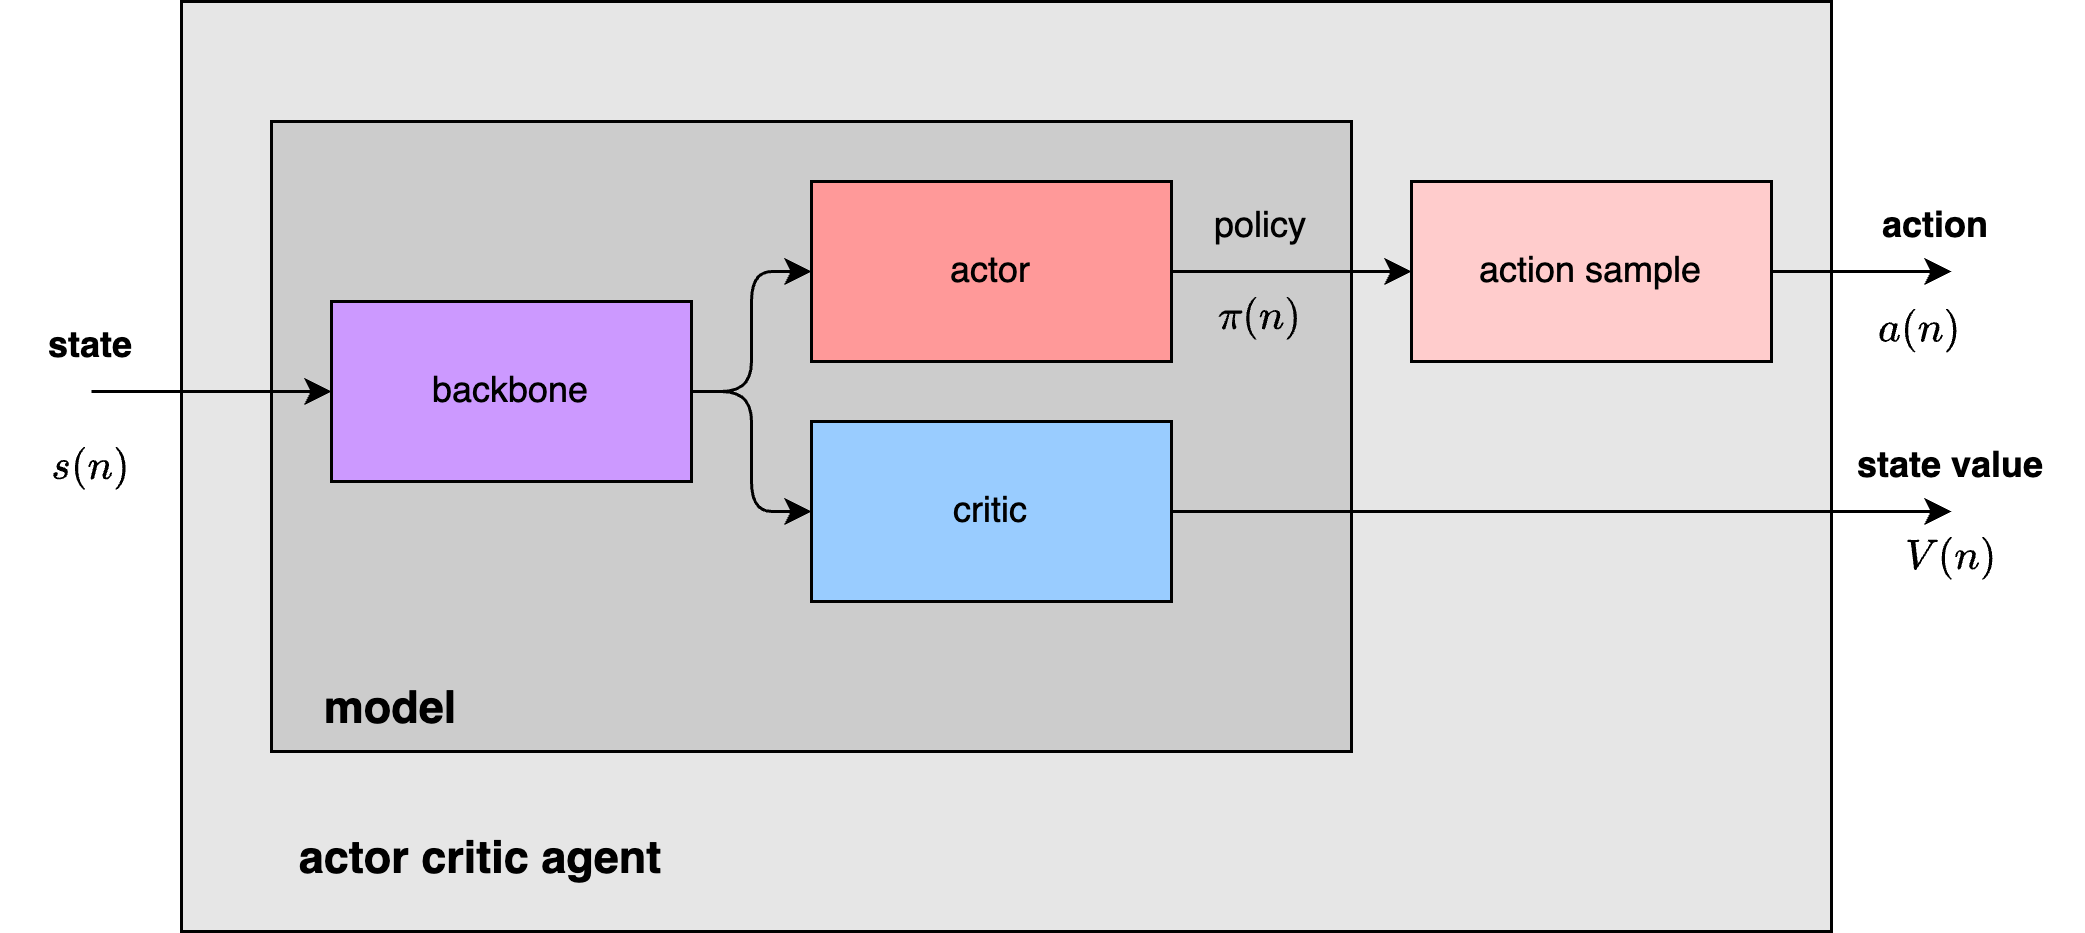
\includegraphics[scale=0.5]
    {../rl_diagrams/a2c-actor_critic_basic.png}

  \vspace{0.1cm}
  \small
  A2C is the simpler learning example; PPO builds on
  similar ideas and adds a more conservative policy update

\end{frame}


\begin{frame}{\bf Action sampling}

  \centering
  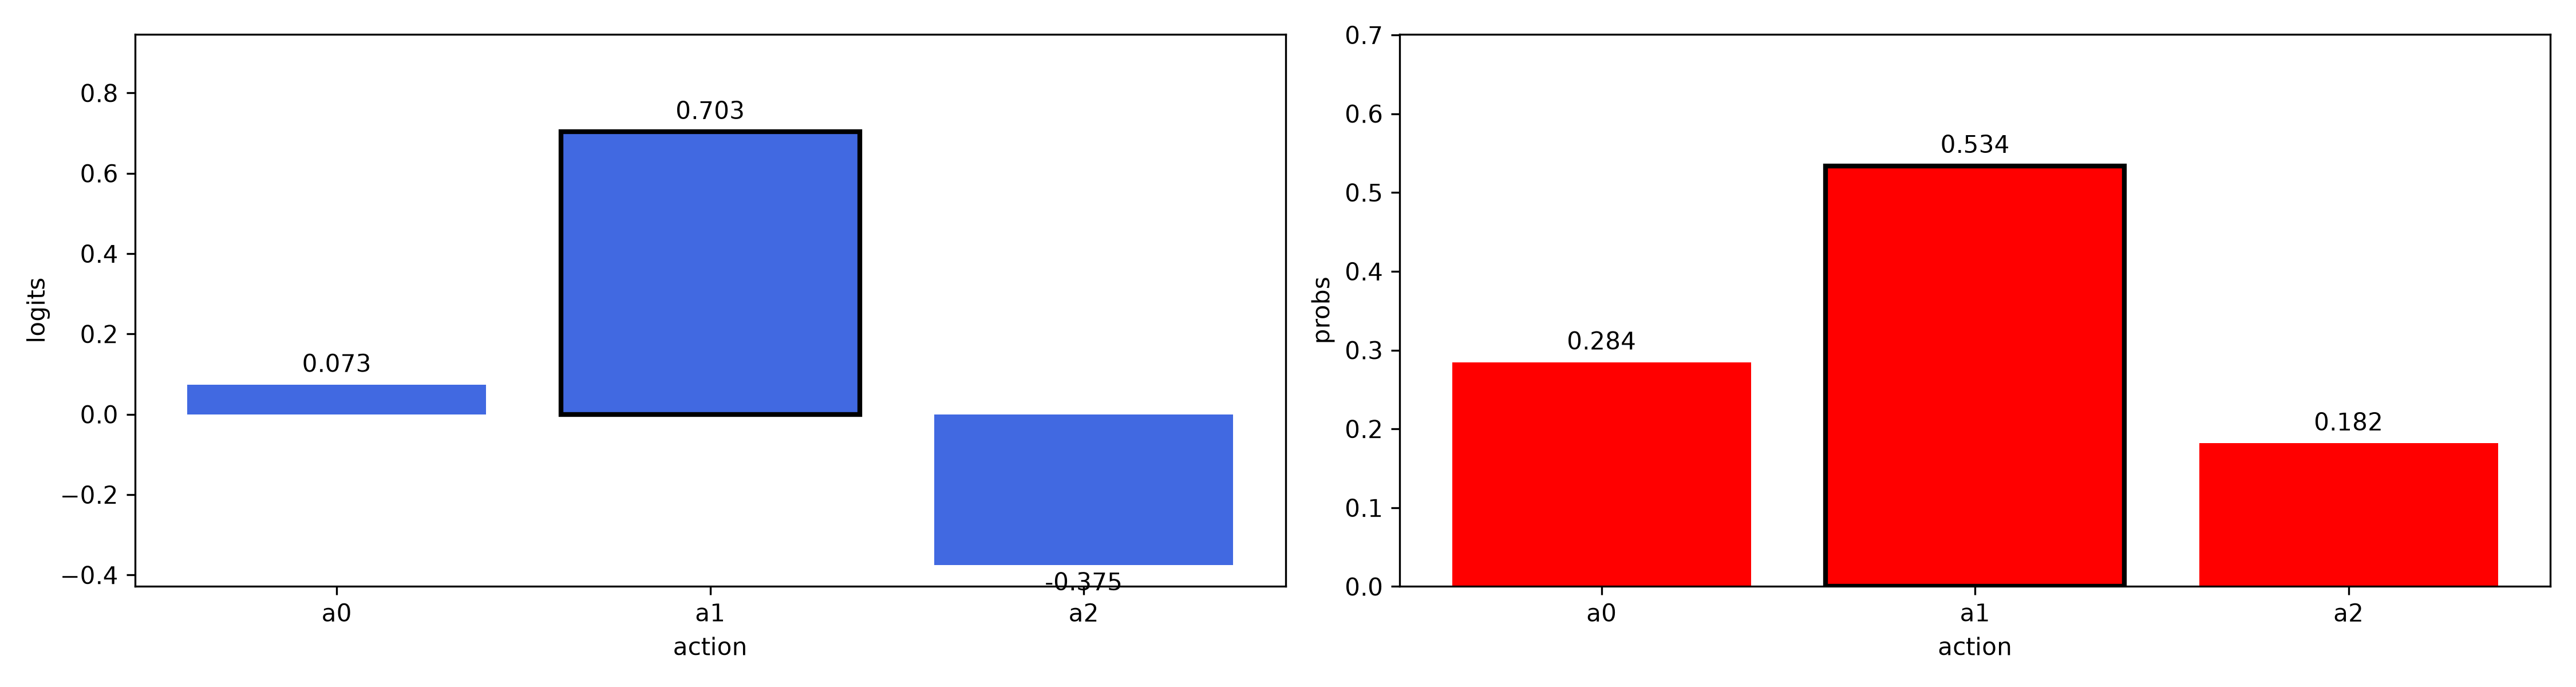
\includegraphics[scale=0.3]
    {../rl_images/a2c_logits_actions.png}

  \begin{enumerate}
    \item \textbf{policy output:}
      $f_\theta(s)$
    \item \textbf{action probabilities:}
      $\pi_\theta(a|s)=\operatorname{softmax}(f_\theta(s))$
    \item \textbf{sample an action:}
      $a\sim\pi_\theta(\cdot|s)$
  \end{enumerate}

  \small
  policy defines a probability distribution over
  available actions \\ during training, sampling encourages
  exploration; \\ during evaluation, we can select the
  highest-probability action

\end{frame}




\begin{frame}{\bf Actor training}

  \centering
  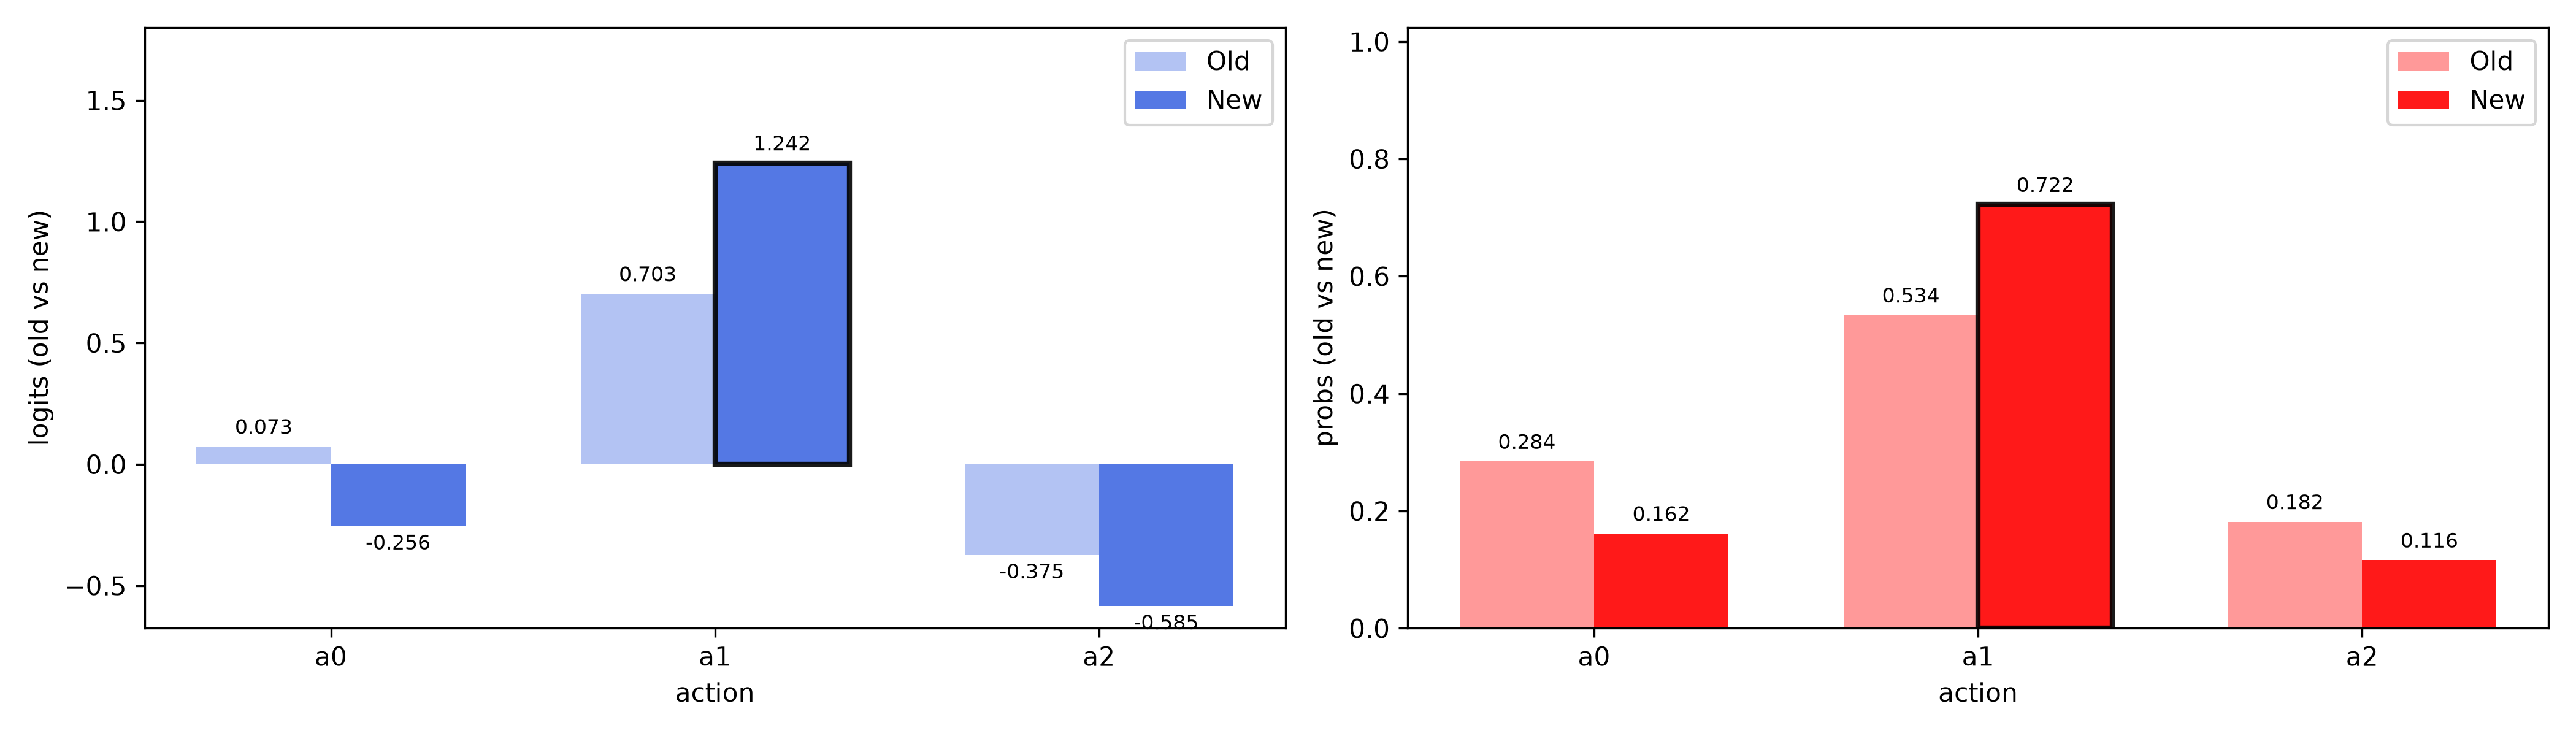
\includegraphics[scale=0.3]
    {../rl_images/a2c_logits_actions_comparison.png}

  \begin{enumerate}
    \item \textbf{advantage:}
      $A(s,a)\approx R-V_\phi(s)$
    \item \textbf{policy loss:}
      $\mathcal{L}_\theta=
      -A(s,a)\log\pi_\theta(a|s)$
  \end{enumerate}

  \small
  positive advantage increases the probability of the
  selected action; negative advantage decreases it \\
  in practice, the return estimate may include multiple
  rewards and bootstrapping from the critic

\end{frame}



\begin{frame}{\bf Critic training}

  \centering
  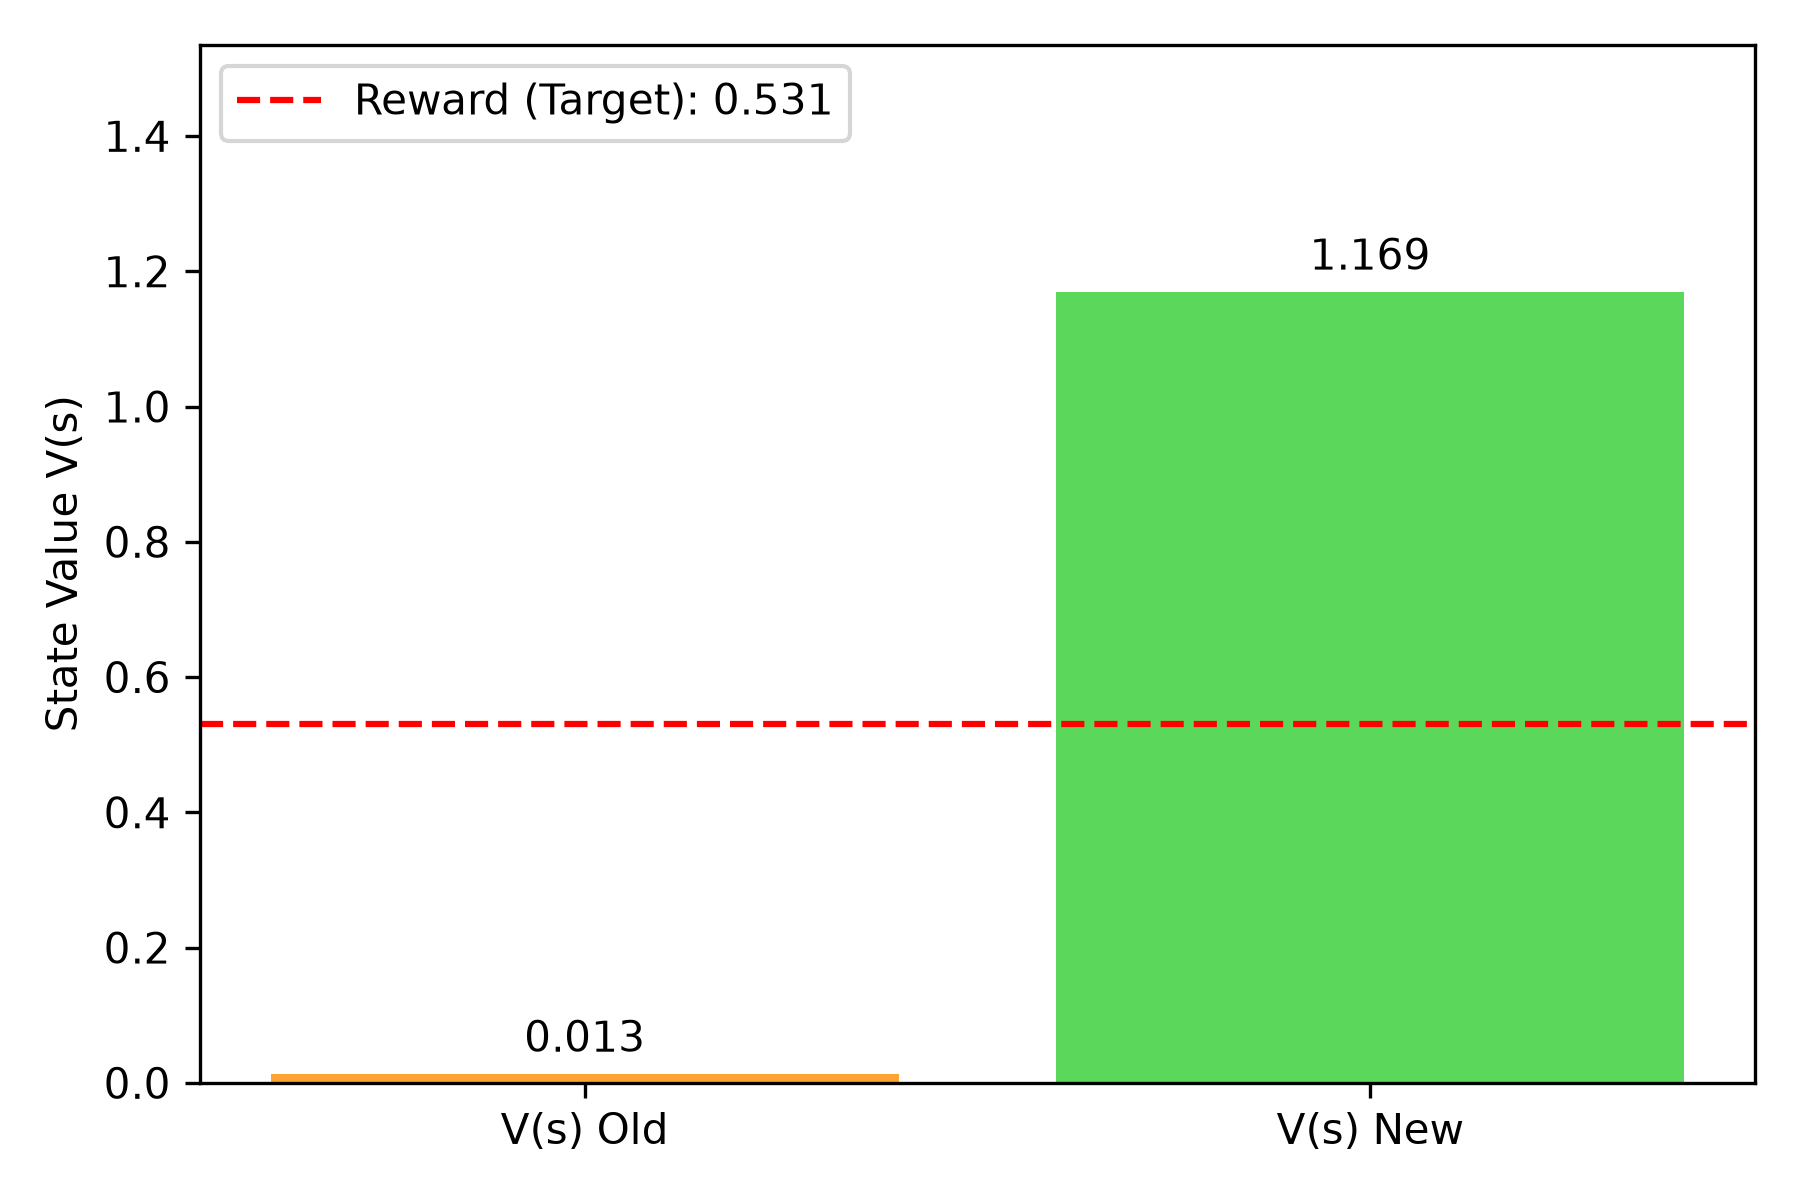
\includegraphics[scale=0.4]
    {../rl_images/a2c_critic_value_comparison.png}

  \begin{enumerate}
    \item \textbf{target return:} $R_t$
    \item \textbf{value prediction:} $V_\phi(s_t)$
    \item \textbf{critic loss:}
      $\mathcal{L}_\phi=
      \big(V_\phi(s_t)-R_t\big)^2$
  \end{enumerate}

  \small
  the critic learns to predict future discounted reward \\
  better value estimates provide a less noisy baseline
  for the actor's policy-gradient updates

\end{frame}





\begin{frame}{\bf A2C training}

  \centering
  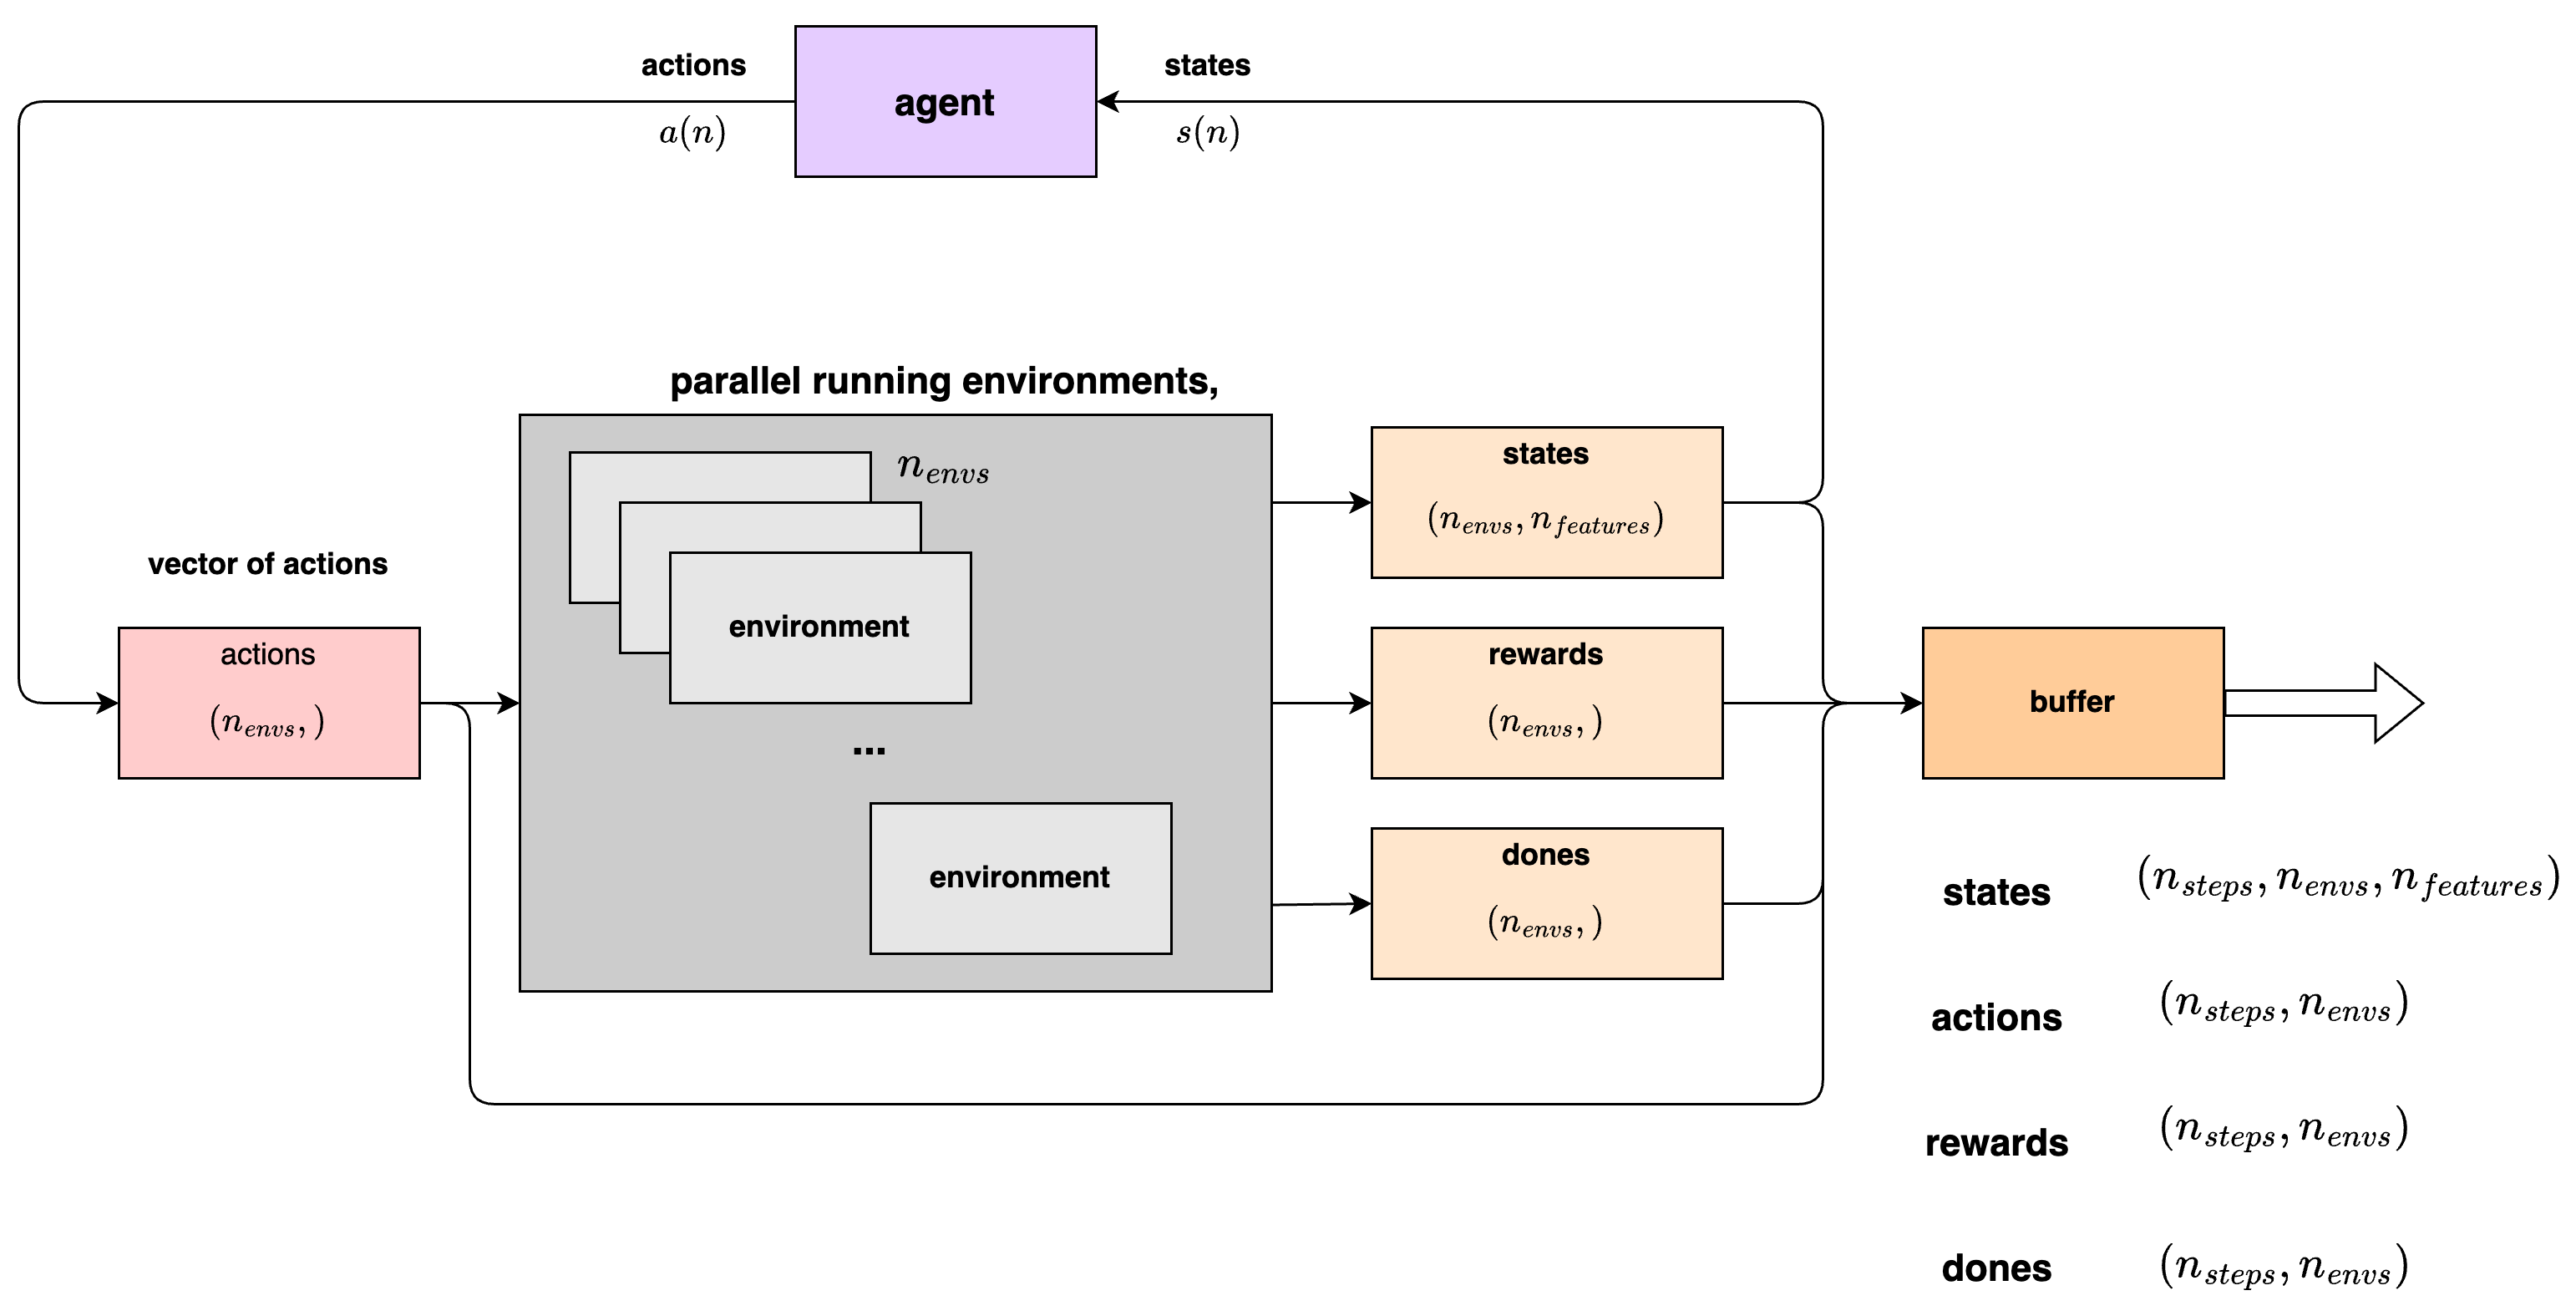
\includegraphics[scale=0.4]
    {../rl_diagrams/a2c-training_01.png}

  \begin{itemize}
    \item collect experience by interacting with the environment
    \item store states, actions, rewards and termination flags
    \item estimate returns and advantages for the collected rollout
  \end{itemize}

\end{frame}


\begin{frame}{\bf A2C training}

  \centering
  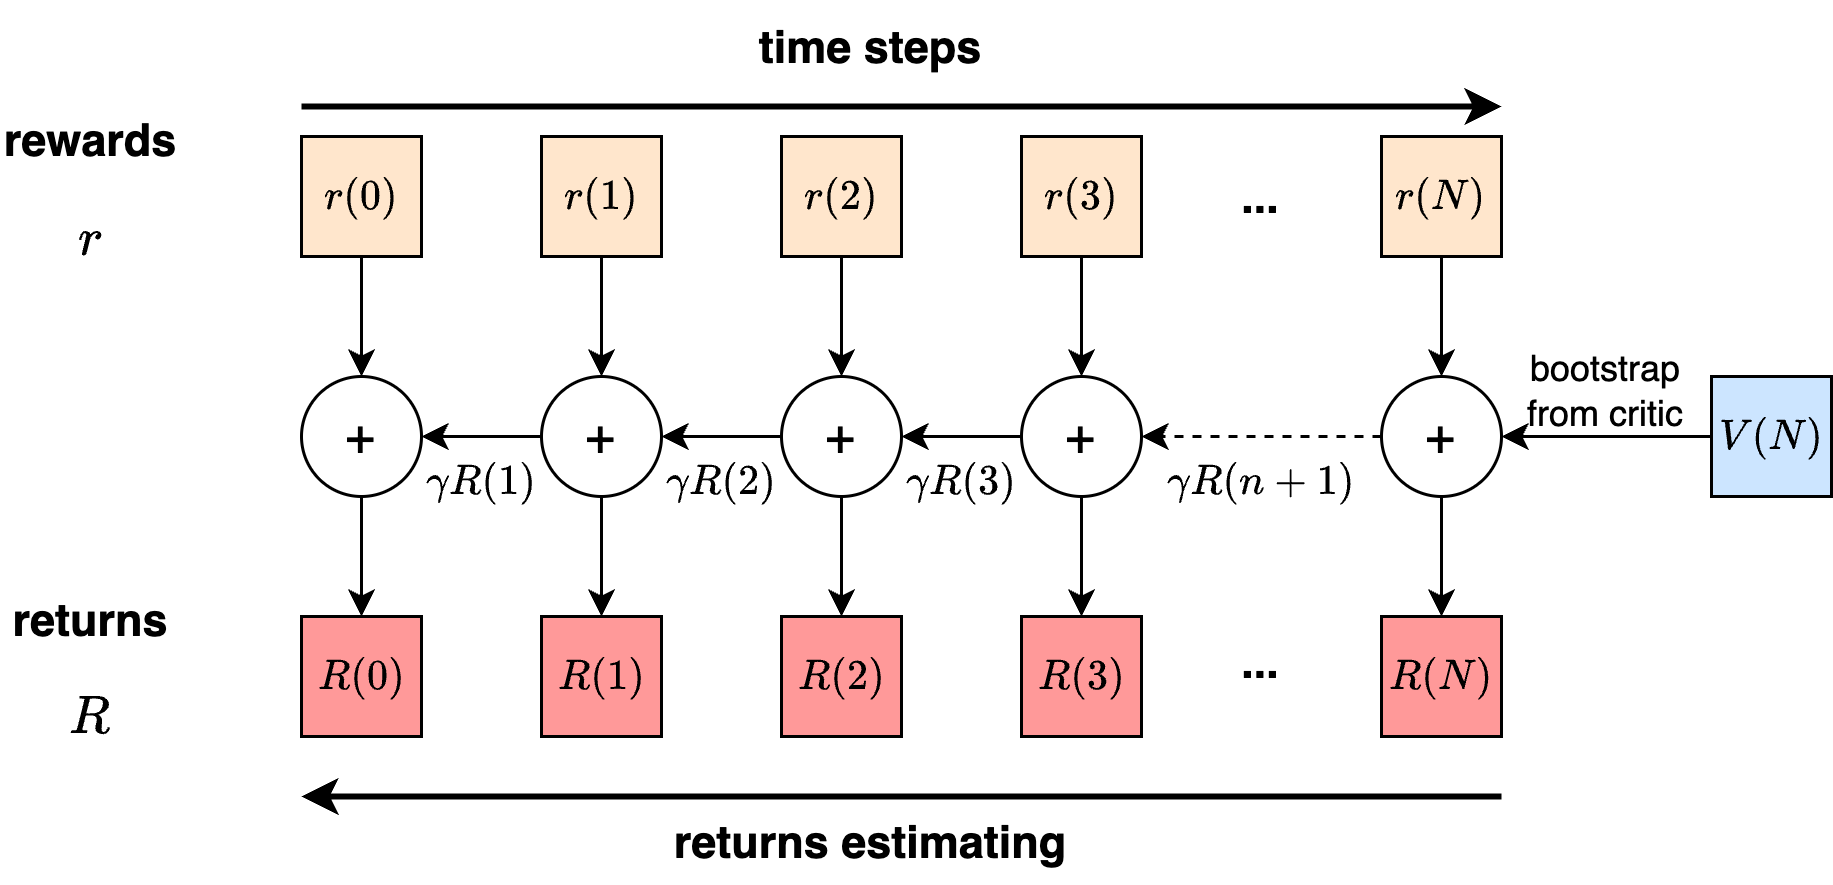
\includegraphics[scale=0.5]
    {../rl_diagrams/a2c-training_02.png}

  \begin{itemize}
    \item estimate \textbf{returns} and \textbf{advantages}
    \item update the  \textbf{actor} using the estimated advantages
    \item update the  \textbf{critic} by minimizing value prediction error
    \item combine policy loss, value loss and an entropy bonus
  \end{itemize}

  \small
  both networks learn from the same experience, but optimize
  different objectives

\end{frame}


\begin{frame}{\bf A2C training}

  \centering
  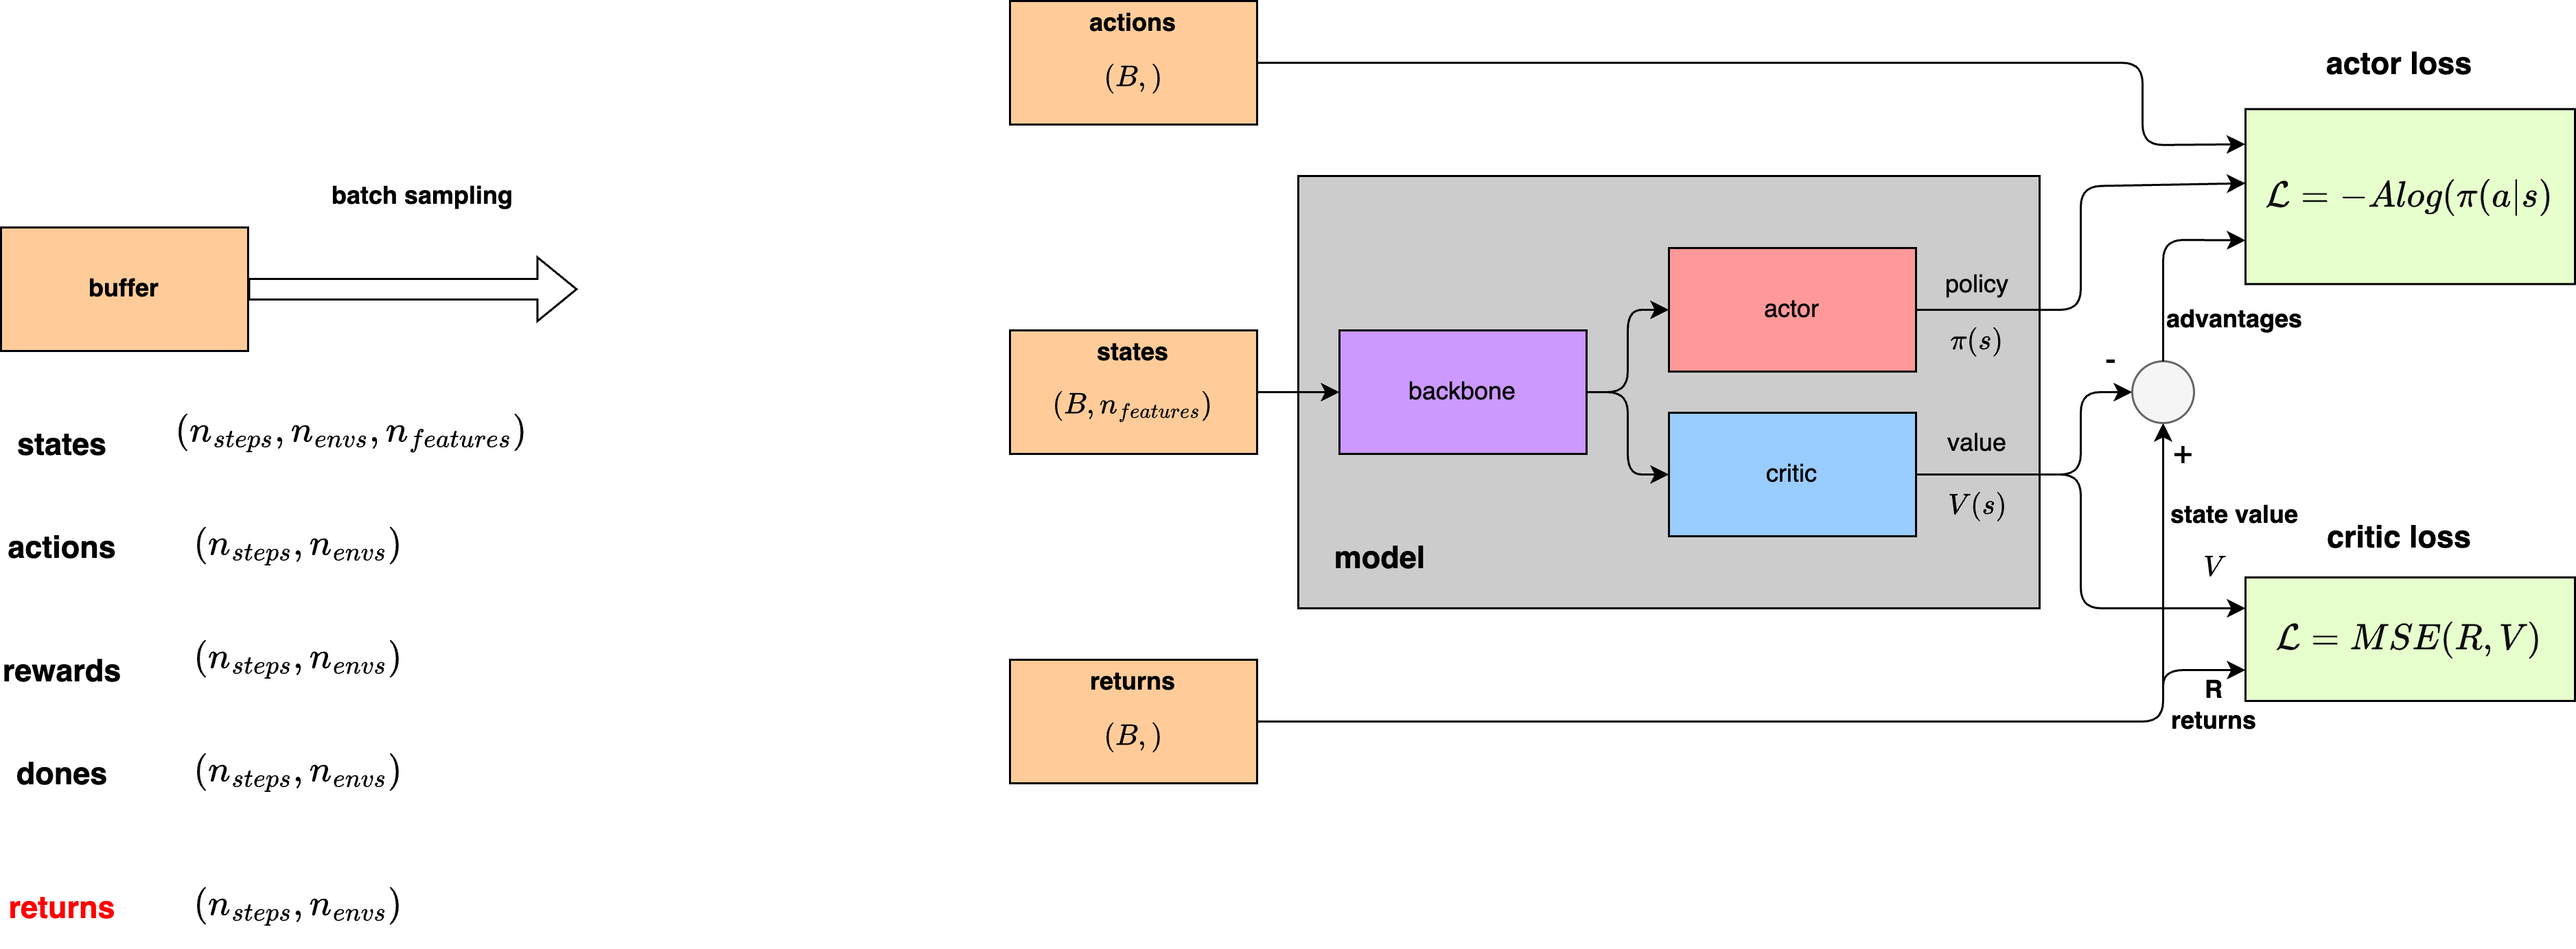
\includegraphics[scale=0.35]
    {../rl_diagrams/a2c-training_03.png}

  \begin{block}{Main takeaway}
    agent learns by repeatedly collecting experience,
    estimating which actions were good, and updating its policy
  \end{block}

\end{frame}






\begin{frame}{\bf Cookbook - choose an environment}

  \begin{itemize}
    \item \textbf{beginner: LunarLander}
      \begin{itemize}
        \item small state vector, discrete actions, clear objective
        \item ideal for understanding A2C and PPO
      \end{itemize}

    \item \textbf{classic games: Atari}
      \begin{itemize}
        \item Breakout, Space Invaders, Pac-Man
        \item practical introduction to image-based RL
      \end{itemize}

    \item \textbf{first-person games: ViZDoom}
      \begin{itemize}
        \item start with \texttt{VizdoomBasic}
        \item then try more complex scenarios and sparse rewards
      \end{itemize}

    \item \textbf{robotics: MuJoCo}
      \begin{itemize}
        \item \texttt{Ant}: locomotion with multiple actuators
        \item \texttt{HalfCheetah}: forward running and speed control
      \end{itemize}
  \end{itemize}

  \vspace{0.1cm}
  \footnotesize
  Official resources:
  \href{https://gymnasium.farama.org/environments/box2d/lunar_lander/}
       {LunarLander},
  \href{https://ale.farama.org/}
       {Atari},
  \href{https://vizdoom.farama.org/}
       {ViZDoom},
  \href{https://gymnasium.farama.org/environments/mujoco/}
       {MuJoCo}.

\end{frame}



\begin{frame}{\bf Cookbook - visual observations}

  \textbf{do not blindly copy the original DQN architecture}

  \begin{itemize}
    \item \textbf{input preprocessing}
      \begin{itemize}
        \item grayscale images to reduce input channels
        \item stack 4 consecutive frames to capture motion
        \item resize to preserve the information needed by the task
      \end{itemize}

    \item \textbf{reasonable starting resolutions}
      \begin{itemize}
        \item Atari: $96\times96$ as an experimental alternative
        \item ViZDoom: $128\times64$ for a wide field of view
      \end{itemize}

    \item \textbf{CNN feature extractor}
      \begin{itemize}
        \item start with 3$\times$3 strided convolutions and 4 layers
        \item flatten the feature map and pass it to an MLP
      \end{itemize}
  \end{itemize}

\end{frame}



\begin{frame}{\bf CNN model example (Atari, Doom ... )}
  \centering
  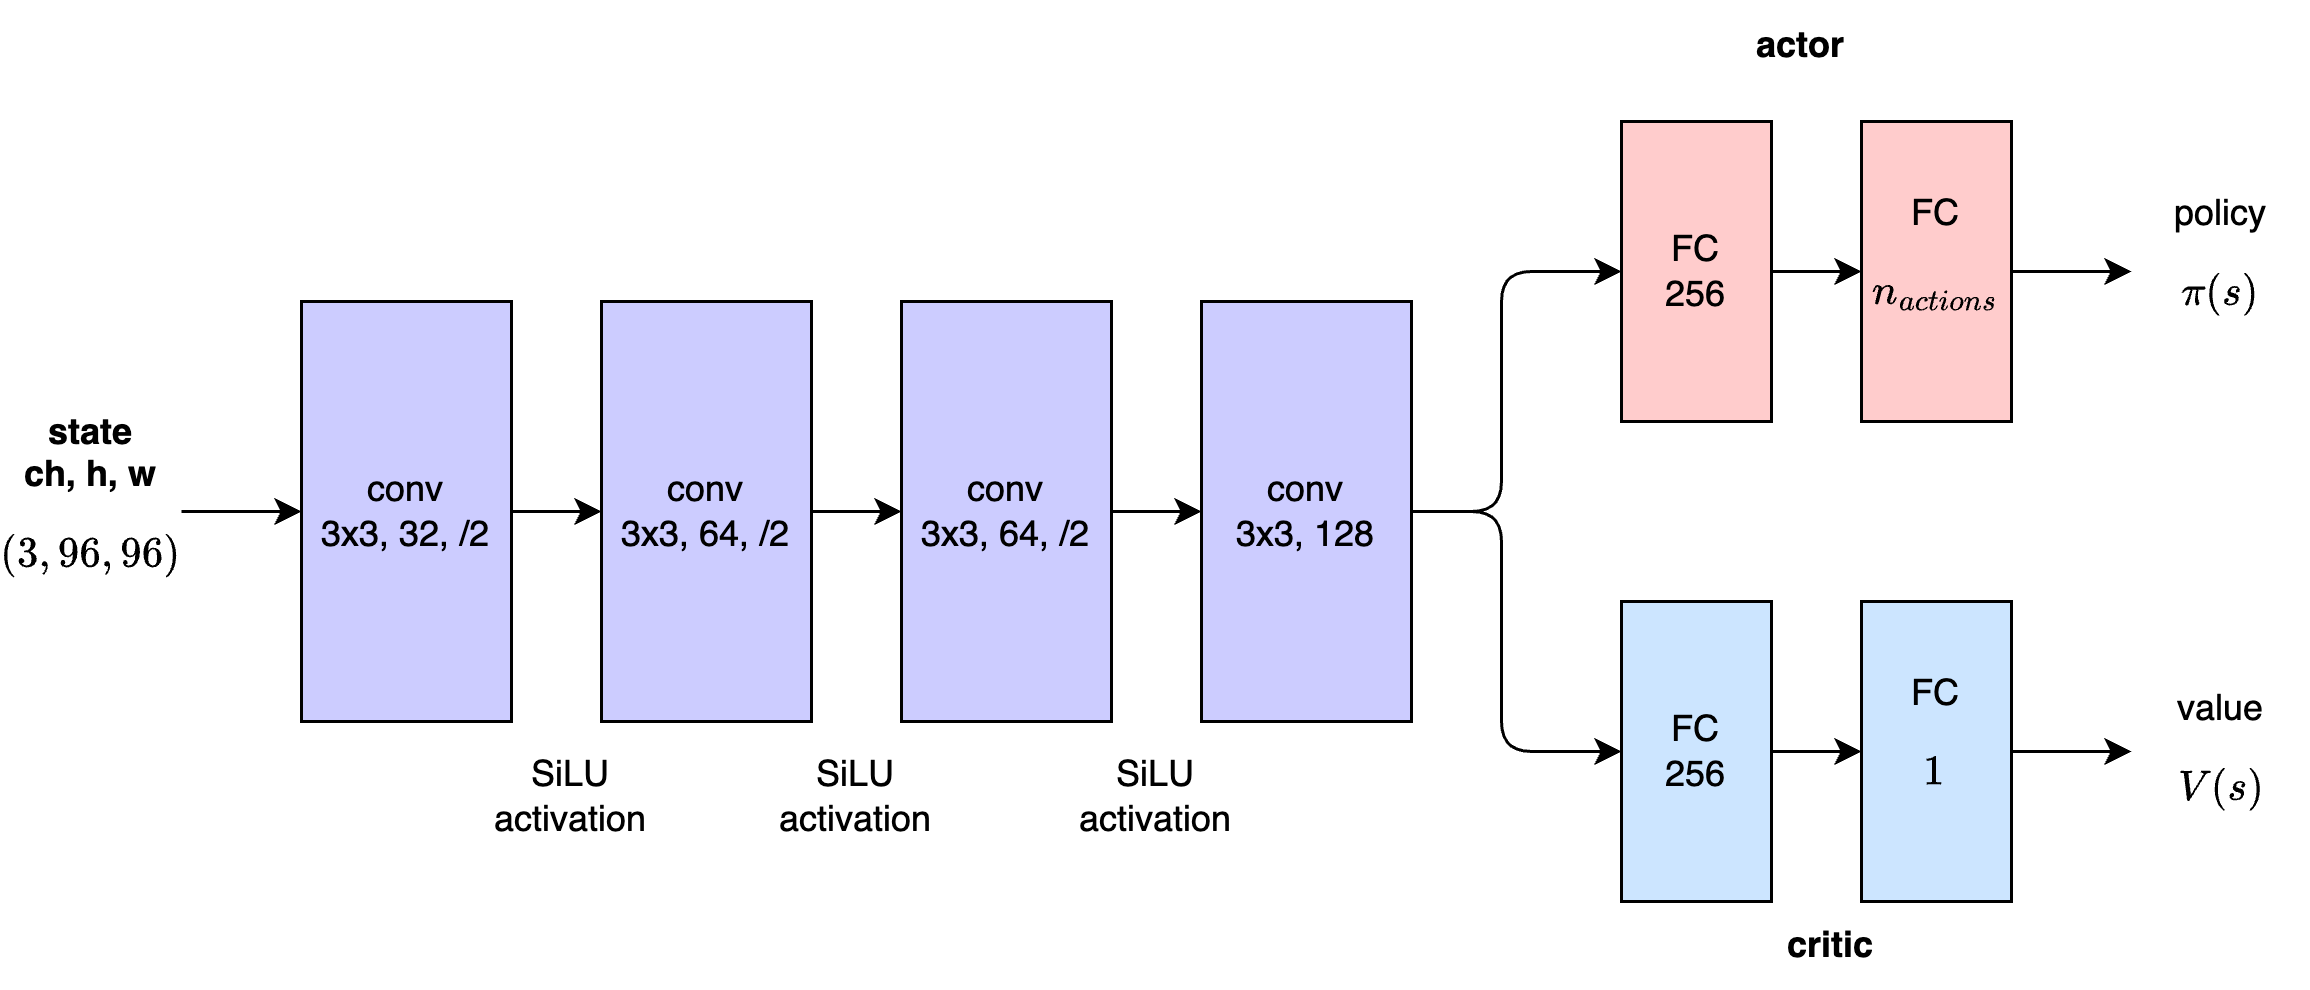
\includegraphics[scale=0.6]{../rl_diagrams/rl_common-cnn_model.png}
\end{frame}


\begin{frame}{\bf MLP model example (Robots, Drones ...)}
  \centering
  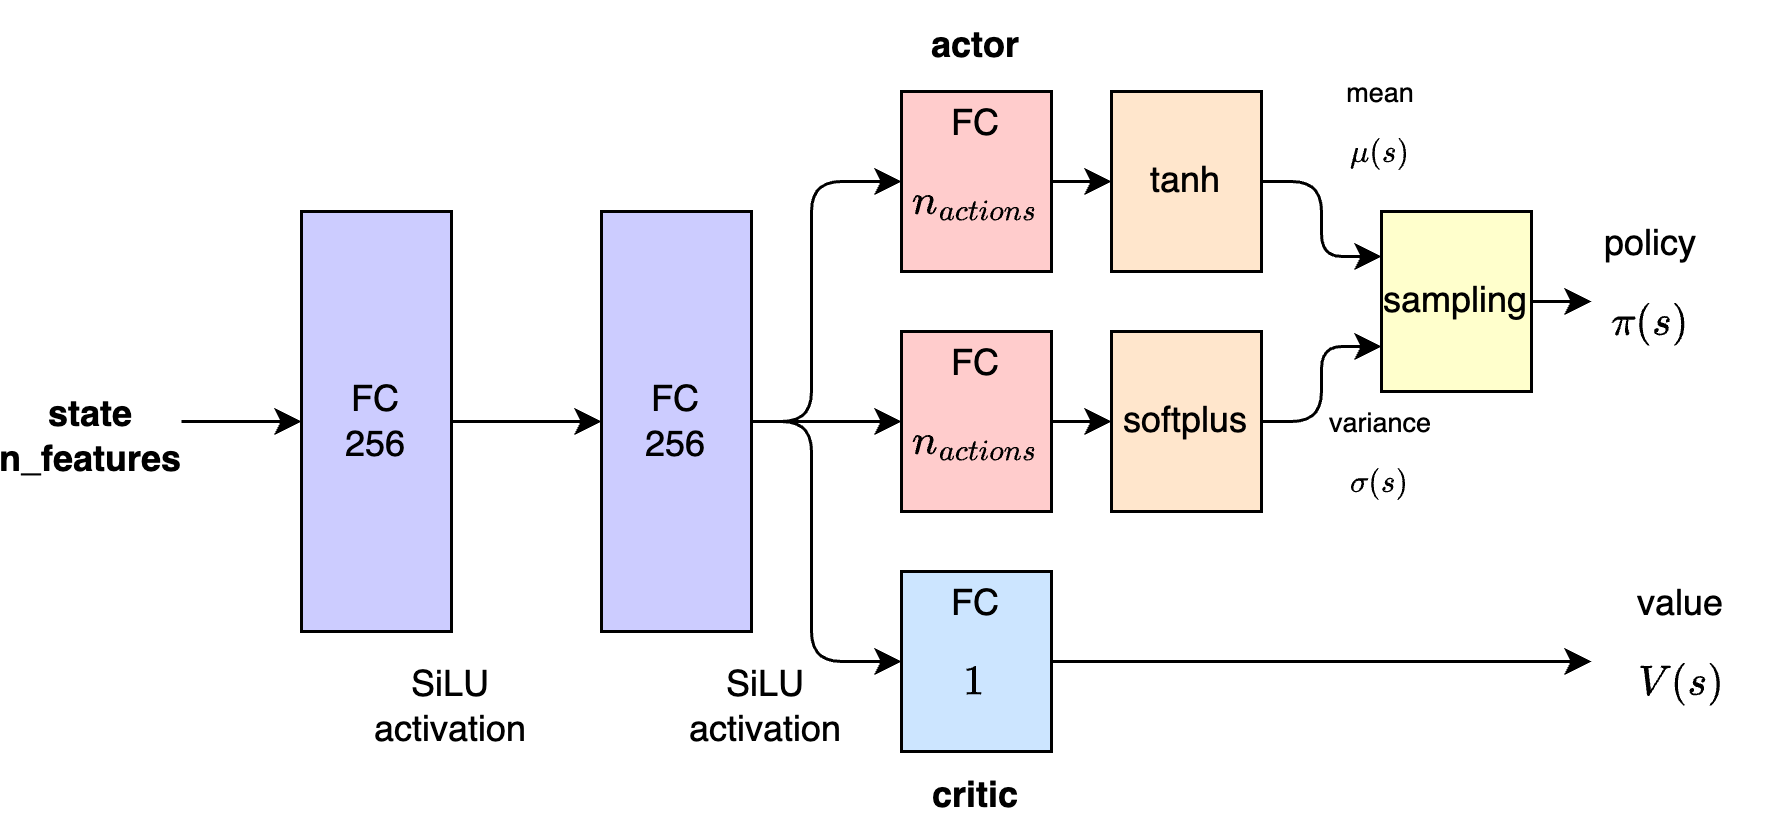
\includegraphics[scale=0.6]{../rl_diagrams/rl_common-mlp_cont_model.png}
\end{frame}




\begin{frame}{\bf main challenges in reinforcement learning}
  \small
  \begin{itemize}
    \item \textbf{\textcolor{cyan}{Sample efficiency}}
      \begin{itemize}
        \item learning may require millions of environment interactions
        \item real robots are slow, expensive, and can be damaged
      \end{itemize}
    \vspace{0.12cm}
    \item \textbf{\textcolor{cyan}{Exploration and sparse rewards}}
      \begin{itemize}
        \item how can an agent discover useful behaviour when success is rare?
        \item poor exploration can leave the policy stuck in local solutions
      \end{itemize}
    \vspace{0.12cm}
    \item \textbf{\textcolor{cyan}{Reward design and alignment}}
      \begin{itemize}
        \item proxy reward may be optimized without achieving the real goal
        \item speed, safety, energy, and task completion may conflict
      \end{itemize}
    \vspace{0.12cm}
    \item \textbf{\textcolor{cyan}{Generalization and robustness}}
      \begin{itemize}
        \item policy that succeeds in training may fail in new conditions
        \item sensor noise, unseen layouts, and changed dynamics matter
      \end{itemize}
  \end{itemize}
  \vspace{0.1cm}
  \begin{alertblock}{Core question}
    can we learn behaviour that is efficient, reliable, and useful beyond the training environment?
  \end{alertblock}
\end{frame}




\begin{frame}{\bf Montezuma's Revenge: exploration with self-supervised distillation}
  \begin{columns}[T,onlytextwidth]
    \begin{column}{0.48\textwidth}
      \centering
      % Replace with a local screenshot if desired:
      % \includegraphics[width=\linewidth]{../images/montezuma_revenge.png}
      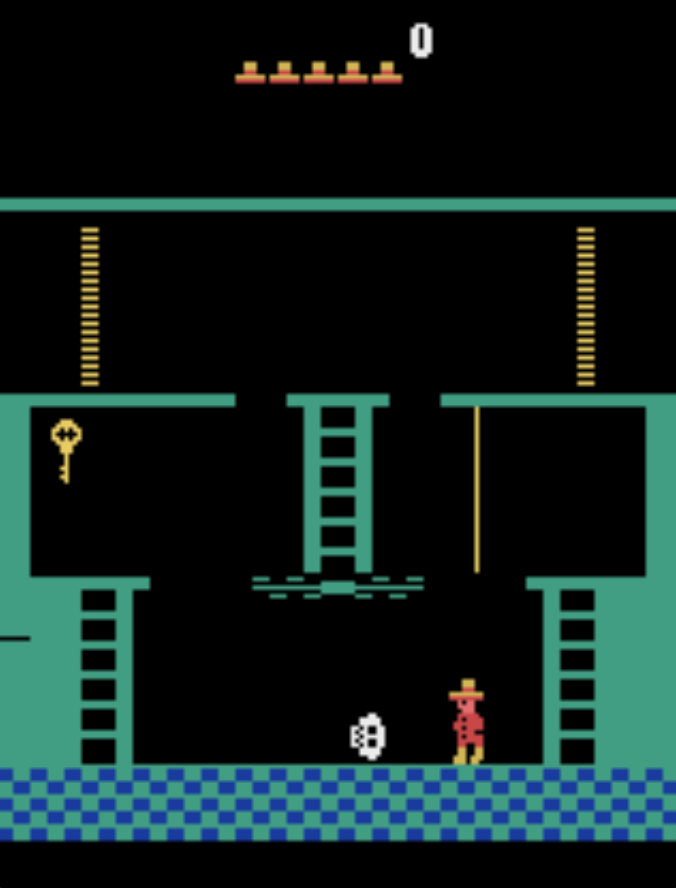
\includegraphics[width=\linewidth]{../images/montezuma.png}
      \vspace{0.1cm}
      \scriptsize
      Montezuma's Revenge: platforms, ladders, hazards, and keys
    \end{column}
    \begin{column}{0.48\textwidth}
      \tiny
      \textbf{The problem}
      \begin{itemize}
        \item rewards are sparse: progress may produce no immediate feedback
        \item the agent must discover unfamiliar states and long action sequences
      \end{itemize}
      \textbf{Self-supervised Network Distillation (SND)}
      \begin{itemize}
        \item predictor learns to match features from a target network
        \item prediction error provides an intrinsic novelty signal
        \item the agent is encouraged to visit states it does not yet represent well
      \end{itemize}
      \begin{block}{Key idea}
        use novelty-driven exploration to discover rewarding behavior when the game itself provides little feedback
      \end{block}
      \vspace{0.05cm}
      \scriptsize
      M. Pecháč, M. Chovanec, I. Farkaš, \emph{Self-supervised network distillation: an effective approach to exploration in sparse reward environments}, Neurocomputing, 2024.
      \href{https://doi.org/10.1016/j.neucom.2024.128033}{doi:10.1016/j.neucom.2024.128033}
    \end{column}
  \end{columns}
\end{frame}


\begin{frame}{\bf Literature - three papers to remember}

  \small

  \textbf{1. DeepMind -- the DQN milestone}

  V. Mnih et al.,

  \textit{Human-level control through deep reinforcement learning}

  Nature, 2015.

  \href{https://www.nature.com/articles/nature14236}
       {nature.com/articles/nature14236}

  \vspace{0.25cm}
  \textbf{2. ETH Zurich -- champion-level drone racing}

  E. Kaufmann et al.,

  \textit{Champion-level drone racing using deep reinforcement learning}

  Nature, 2023.

  \href{https://www.nature.com/articles/s41586-023-06419-4}
       {nature.com/articles/s41586-023-06419-4}

  \vspace{0.25cm}
  \textbf{3. Self-supervised Network Distillation (SND)}

  M. Pecháč, M. Chovanec, I. Farkaš,

  \textit{Self-supervised network distillation: an effective
  approach to exploration in sparse reward environments}

  Neurocomputing, 2024.

  \href{https://doi.org/10.1016/j.neucom.2024.128033}
       {doi:10.1016/j.neucom.2024.128033}

\end{frame}




\begin{frame}{\bf Literature - further reading}

  \small

  \textbf{Actor--Critic and asynchronous learning}

  V. Mnih et al.,

  \textit{Asynchronous Methods for Deep Reinforcement Learning}

  ICML, 2016.

  \href{https://proceedings.mlr.press/v48/mniha16.html}
       {PMLR: A3C paper}

  \vspace{0.2cm}
  \textbf{Practical policy optimization}

  J. Schulman et al.,

  \textit{Proximal Policy Optimization Algorithms}

  arXiv, 2017.

  \href{https://arxiv.org/abs/1707.06347}
       {arXiv:1707.06347}

  \vspace{0.2cm}
  \textbf{Continuous control and sample efficiency}

  T. Haarnoja et al.,

  \textit{Soft Actor-Critic Algorithms and Applications}

  arXiv, 2018.

  \href{https://arxiv.org/abs/1812.05905}
       {arXiv:1812.05905}

  \vfill
  \hrule
  \vspace{0.1cm}

  \footnotesize
  \textbf{Theory:} PPO builds on policy-gradient and
  trust-region ideas. Read the PPO paper for the clipped
  objective, surrogate loss and empirical comparisons.

\end{frame}




\begin{frame}{\bf policy gradient: learning from samples}
\begin{itemize}
    \item our goal is to \textbf{\textcolor{cyan}{maximize}} the expected return:
    \[
        J(\theta)=\mathbb{E}_{\tau\sim\pi_\theta}[R(\tau)].
    \]
    \item in practice, \textbf{\textcolor{red}{we do not know the exact distribution}} of all possible trajectories
    \item instead, we collect trajectories by running the policy and use a \textbf{Monte Carlo} estimate:
    \[
        J(\theta)\approx \frac{1}{N}\sum_{i=1}^{N}R(\tau_i).
    \]
    \item to improve the policy, we need the gradient $\nabla_\theta J(\theta)$
\end{itemize}
\end{frame}

\begin{frame}{\bf policy gradient: the log trick}
we only  \textbf{have sampled trajectories}, so we want a gradient we can estimate from those samples

\[
\begin{aligned}
\nabla_\theta J(\theta)
&= \nabla_\theta \mathbb{E}_{\tau\sim\pi_\theta}[R(\tau)]\\
&= \mathbb{E}_{\tau\sim\pi_\theta}
   \left[R(\tau)\nabla_\theta\log P(\tau;\theta)\right]
\end{aligned}
\]

\begin{itemize}
    \item \textbf{\textcolor{cyan}{the key identity is}}
    \[
        \nabla_\theta P(\tau;\theta)
        =P(\tau;\theta)\nabla_\theta\log P(\tau;\theta)
    \]
    \item it turns the gradient of a probability into a log-probability gradient that we can evaluate for sampled trajectories
    \item since the environment's dynamics do not depend on $\theta$,
    \[
        \nabla_\theta\log P(\tau;\theta)
        =\sum_t\nabla_\theta\log\pi_\theta(a_t\mid s_t)
    \]
\end{itemize}

\[
\nabla_\theta J(\theta)\approx
\frac{1}{N}\sum_{i=1}^{N}R(\tau_i)
\sum_t\nabla_\theta\log\pi_\theta(a_{i,t}\mid s_{i,t})
\]
\end{frame}




\begin{frame}{REINFORCE: learning from discounted returns}
    for each time step, define the \textbf{\textcolor{cyan}{discounted return}}:
    \[
        G_t = \sum_{k=0}^{T-t-1} \gamma^k r_{t+k+1}
    \]

    \vspace{-0.1cm}
    return measures the rewards collected after taking action
    $a_t$ in state $s_t$, with future rewards discounted by $\gamma$.

    \vspace{0.2cm}
    REINFORCE gradient estimator is
    \[
        \hat{g}
        =
        \frac{1}{N}
        \sum_{i=1}^{N}
        \sum_{t=0}^{T_i-1}
        G_t^{(i)}
        \nabla_\theta
        \log \pi_\theta(a_t^{(i)} \mid s_t^{(i)}).
    \]

    \begin{itemize}
        \item collect trajectories using the current policy
        \item compute the discounted return $G_t$ for each action
        \item increase the probability of actions followed by high returns;
              decrease it for actions followed by low returns
    \end{itemize}
\end{frame}


\begin{frame}{REINFORCE: the problem of high variance}
    return $G_t$ is a \textbf{\textcolor{red}{noisy estimate of how good an action was}}

    \vspace{0.2cm}
    \begin{itemize}
        \item \textbf{different outcomes:}
              similar states and actions can lead to very different
              future rewards
        \item \textbf{delayed rewards:}
              an outcome may depend on many later actions
        \item \textbf{noisy updates:}
              different sampled trajectories can suggest very different
              parameter updates
    \end{itemize}

    
    \vspace{0.2cm}
    \textbf{consequence:} REINFORCE gives an unbiased gradient estimate,
    but its high variance can make learning slow and unstable
\end{frame}


\begin{frame}{Reducing variance: critic and advantages}
    critic estimates how much \textbf{\textcolor{cyan}{future reward we expect from a state}}
    under the current policy :
    \[
        V^\pi(s_t)
        =
        \mathbb{E}_\pi[G_t \mid s_t].
    \]


    instead of using the return directly, we compute the \textbf{\textcolor{red}{advantage}}:
    \[
        \hat{A}_t = G_t - V_\phi(s_t).
    \]

    \vspace{-0.1cm}
    actor update becomes
    \[
        \hat{g}
        =
        \sum_t
        \hat{A}_t
        \nabla_\theta
        \log \pi_\theta(a_t \mid s_t).
    \]


    \begin{itemize}
        \item $\hat{A}_t > 0$: \textbf{\textcolor{cyan}{the outcome was better than expected}};
              increase the action's probability
        \item $\hat{A}_t < 0$: \textbf{\textcolor{red}{the outcome was worse than expected}};
              decrease the action's probability
        \item $\hat{A}_t \approx 0$: \textbf{\textcolor{green}{the outcome was close to expectation}};
              make little change.
    \end{itemize}

    
\end{frame}




\begin{frame}{\bf Q\&A}


\url{michal.nand@gmail.com}

\url{https://github.com/michalnand/lectures/}

 
\end{frame}


\end{document}
